\documentclass{mythesis}

\usetikzlibrary{decorations.markings}
\usetikzlibrary{hobby}
\usepackage{pgfplots}
\pgfplotsset{compat=1.11}

\DeclareDocumentCommand{\Ind}{}{\operatorname{Ind}}
\DeclareDocumentCommand{\S}{}{\mathbb{S}}
\DeclareDocumentCommand{\lc}{}{\operatorname{lc}}
\DeclareDocumentCommand{\rem}{}{\operatorname{rem}}

\usepackage{stmaryrd}

\ExplSyntaxOn
\DeclareDocumentCommand { \Index } { m m m } {
    \mathopen{\llbracket} #2 \mathbin{:} \nobreak #3 \mathclose{\rrbracket\c_math_subscript_token{\mathsmaller{#1}}}
}
\DeclareDocumentCommand { \IndexP } { m m } {
    \mathopen{\llbracket} #1 \mathbin{:} \nobreak #2 \mathclose{\rrbracket}
}
%\DeclareDocumentCommand { \Index0 } { m m } {
%    \mathopen{\llbracket} #1 \mathclose{\rrbracket\c_math_subscript_token{\mathsmaller{#2}}}
%}
\ExplSyntaxOff

%\usepackage[authoryear]{natbib}
%\renewcommand{\cite}[1]{\citealp{#1}}

\usepackage{titling}

\title{Der reell-algebraische Abbildungsgrad}
\author{Stephan Hilb}

\begin{document}

\begin{titlepage}
    \begin{center}
        ~\par\vspace{5em}
        {
            \fontsize { 18pt } { 18pt } \selectfont
            Bachelorarbeit
        }
        \par\vspace{3em}
        {
            \fontsize { 26pt } { 26pt } \selectfont \sffamily \bfseries
            \thetitle
        }
        \par\vspace{3em}
        {
            \fontsize { 16pt } { 16pt } \selectfont \scshape
            \theauthor
        }
        \par\vspace{1.5em}
        {
            \fontsize { 14pt } { 14pt } \selectfont %\scshape
            \today
        }
        \par\vspace{3.5em}
        {
        \begin{tikzpicture}[
            scale=1.3,
            decoration={ markings, mark=between positions 0.1 and 1 step 2.5cm with {\arrow{stealth}} }
        ]
            \draw[->] (-2,0) to (5.3,0) node[anchor=south east] {$x$};
            \draw[->] (0,-1.1) to (0,1.4) node[anchor=north west] {$y$};
            \coordinate (z0) at (-1.5,0);
            \coordinate (z1) at (1.2,0);
            \coordinate (z2) at (3,0);
            \coordinate (z3) at (4.5,0);
            \draw[closed hobby,draw=main1, postaction={decorate} ] plot coordinates
                { (z0) (0,-0.8) (z1) (2,0.5) (z2) (3.8,-0.4) (z3) (3.5,1) (0,0.8) };
            \node[anchor=45] at (z0) {$+1$};  %\fill[hl1] (z0) circle (1pt);
            \node[anchor=100] at (z1) {$+1$}; %\fill[hl1] (z1) circle (1pt);
            \node[anchor=60] at (z2) {$-1$};  %\fill[hl1] (z2) circle (1pt);
            \node[anchor=120] at (z3) {$+1$}; %\fill[hl1] (z3) circle (1pt);
        \end{tikzpicture}
        }
        \par
        {
\pgfplotsset{
    colormap={red}{rgb255(0cm)=(240,160,160); rgb255(1cm)=(240,160,160)},
    colormap={greenyellow}{rgb255(0cm)=(0,128,0); rgb255(1cm)=(255,255,0)},
    colormap={greenyellow2}{rgb255(0cm)=(128,128,0); rgb255(1cm)=(0,255,0)},
}
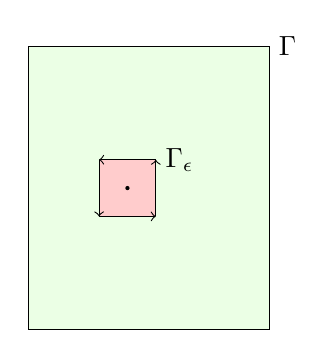
\begin{tikzpicture}[scale=1.8,baseline=(current bounding box.center)]
    %\draw[->,thin] (0,0) -- (10,0) node[anchor=135] {$x$};
    %\draw[->,thin] (0,0) -- (0,10) node[anchor=0] {$y$};
    \draw[fill=green!80!yellow!10] (-0.7,-1) rectangle (1,1) node[right] {$\Gamma$};
    %\coordinate[label={below:$(x_0,y_0)$}] (p) at (4,3);
    \coordinate (p) at (0,0);
    \pgfmathsetmacro{\geps}{0.2};
    \path[fill=red!20] (p) +(-\geps,-\geps) rectangle +(\geps,\geps) node[right] {$\Gamma_\epsilon$};
    \fill (p) circle (0.1ex);
    \path (p)
        +(-\geps,-\geps) edge[->] +(\geps,-\geps)
        +(\geps,-\geps) edge[->] +(\geps,\geps)
        +(\geps,\geps) edge[->] +(-\geps,\geps)
        +(-\geps,\geps) edge[->] +(-\geps,-\geps);
\end{tikzpicture}
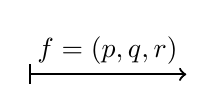
\begin{tikzpicture}
    \path[|->,thick] (-1,0) edge (1,0);
    \node[anchor=-90] at (0,0) {$f = (p,q,r)$};
\end{tikzpicture}
\begin{tikzpicture}[baseline=(current bounding box.center)]
    \begin{axis} [
        hide axis,
        view={-10}{35},
        xmin=-3,xmax=2.3,
        ymax=2.5,
    ]
        \draw[->] (0,0,0) -- (2.1,0,0) node[below] {$p$};
        \addplot3 [
            raw gnuplot,
            parametric,
            surf,
            %shader=flat,
            colormap name=greenyellow,
        ] gnuplot {
            set parametric;
            set hidden3d;
            set isosamples 31,31;
            set urange [-0.7:0.8];
            set vrange [-1:1];
            splot u-v+u*v/3,v+u/2-v*(1-u)/3,u*u*u*u/0.7 + 2*u*u*(u-1) + u + v*v
        };
        \addplot3 [
            raw gnuplot,
            parametric,
            surf,
            %shader=flat,
            colormap name=red,
        ] gnuplot {
            set parametric;
            set hidden3d;
            set isosamples 7,7;
            set urange [-0.2:0.2];
            set vrange [-0.2:0.2];
            splot u-v+u*v/3,v+u/2-v*(1-u)/3,u*u*u*u/0.7 + 2*u*u*(u-1) + u + v*v
        };
        \draw[->] (-2.5,0,0) -- (-2.5,-2,0) node[below left] {$q$};
        \draw[->] (-2.5,0,0) -- (-2.5,0,3) node[left] {$r$};
        \draw (-2.5,0,0) -- (0,0,0);
        \fill (0,0,0) circle (0.2ex);
    \end{axis}
\end{tikzpicture}
        }
        \par\vspace{8em}
        {
            \fontsize { 14pt } { 14pt } \selectfont \scshape
            Universität Stuttgart
        }
        \par\vspace{1em}
        {
            \fontsize { 14pt } { 14pt } \selectfont %\scshape
            Institut für Geometrie und Topologie
        }
        \par\vspace{1em}
        {
            \fontsize { 14pt } { 14pt } \selectfont %\scshape
            Betreuer: Prof. Dr. Michael Eisermann
        }
    \end{center}
\end{titlepage}

\chapter*{Übersicht}

Die Windungszahl einer polynomiellen Kurve $\gamma: [0, 1] \to \C^*$ lässt sich als halben Cauchy-Index der rationalen Funktion $\frac{\Re \gamma}{\Im \gamma}$ auf $[0,1]$ definieren, was anschaulich gesprochen die Überquerungen der Kurve an der rellen Achse mit $\pm \frac{1}{2}$ zählt.
Ein reell-algebraischer Algorithmus, basierend auf polynomieller Restbildung oder sogenannten Sturm-Ketten, erlaubt die explizite Berechnung dieses Cauchy-Index und damit auch der Windungszahl von $\gamma$.

Im ersten Kapitel betrachten wir diese Erkenntnisse von Cauchy und Sturm aus einem neuen Blickwinkel, der es uns erlaubt im zweiten Kapitel einen ähnlichen Algorithmus für den Abbildungsgrad als Verallgemeinerung der Windungszahl in zwei Variablen beschreiben und untersuchen zu können.


{
    \let\clearpage\relax
    \tableofcontents
    %\addtocentrydefault{chapter}{}{Inhaltsverzeichnis}
}
%\tableofcontents


\clearpage
\chapter{Der univariate Fall: Windungszahl und Cauchy-Index} \label{sec:1}

\section{Geometrische Motivation}

Sei $\gamma: [a,b] \to \C$ eine geschlossene Kurve.
Mit $\deg(\gamma) \in \Z$ bezeichnen wir die Anzahl Umläufe von $\gamma$ um die Null, wobei wir Umläufe entgegen dem Uhrzeigersinn positiv und solche im Uhrzeigersinn negativ werten.
Die Zahl $\deg(\gamma)$ besitzt den treffenden Namen \emph{Windungszahl}, ein Beispiel findet sich in \ref{fig:winding_number}.

\begin{figure}[ht]
    \centering
    \begin{tikzpicture}[
        xscale=1.5,
        decoration={ markings, mark=between positions 0 and 1 step 2.3cm with {\arrow{stealth}} },
    ]
        \draw[->] (-2,0) to (2.1,0) node[anchor=south east] {$x$};
        \draw[->] (0,-1.5) to (0,1.5) node[anchor=north west] {$y$};
        \draw[closed hobby,draw=main1, postaction={decorate} ] plot coordinates
            { (1.5,0.5) (0,1) (-1.5,0.5) (-1.0,-0.8) (1,-0.6) (0,0.5) (-0.5,-0.5) (1.5,-0.6) };
    \end{tikzpicture}
    \caption{Kurve mit Windungszahl $\deg(\gamma) = 2$}
    \label{fig:winding_number}
\end{figure}

Formalisieren lässt sich die Windungszahl auf viele verschiedene Arten und Weisen.
Eine traditionelle Idee hierfür ist das Aufsummieren der Winkel, die beim Durchlaufen der Kurve mit dem Ursprung eingeschlossen werden.
Die Topologie stellt beispielsweise simpliziale Approximation bereit, um die Winkelzählung auf eine endliche Summation zu reduzieren.
% fixme: cite: wie in \cite[§I1f,§I1h]{eiserm_topology}
Im Analysis-Werk \cite[§12.7]{koenigsberger2003analysis} wird der Begriff der \emph{Liftung} eingeführt, um die Winkeländerung zu erfassen.
Abgesehen davon hat die Windungszahl auch eine Integraldarstellung $\frac{1}{2\pi i} \int_{\gamma} \frac{1}{z} \di[z]$, die in der komplexen Analysis sehr gebräuchlich ist.
% fixme: Siehe dazu beispielsweise \cite{??}.

Für unsere Zwecke werden wir uns auf (stückweise) polynomielle Kurven beschränken und können daher eine einfachere und zugleich intuitive Definition wählen.

\begin{definition}
    Seien $p, q \in \R[x]$ und $a, b \in \R$, $a < b$.
    Wir nennen $\gamma: [a, b] \to \C$ mit $\gamma(t) = p(t) + iq(t)$ eine \emphdef{polynomielle Kurve}.
\end{definition}

Für eine polynomielle Kurve $\gamma: [a,b] \to \C^*$ ohne Nulldurchgang realisieren wir die Zählung der Umläufe $\deg(\gamma)$, indem wir ihre Übergänge über die reelle Achse betrachten.
In \ref{fig:curve_counting_example} zählen wir solche Übergänge einer geschlossenen Kurve mit ihrer Orientierung und erhalten in der Summe $1 + 1 - 1 + 1 = 2$.
Die Umläufe der Kurve werden so doppelt gezählt: auf der negativen und auf der positiven reellen Achse, die Windungszahl der Kurve beträgt unterdessen $\deg(\gamma) = 1$.

\begin{figure}[ht]
    \centering
    \begin{subfigure}[t]{0.49\textwidth}
        \centering
        \begin{tikzpicture}[
            decoration={ markings, mark=between positions 0.1 and 1 step 2.5cm with {\arrow{stealth}} }
        ]
            \draw[->] (-2,0) to (5.3,0) node[anchor=south east] {$x$};
            \draw[->] (0,-1.1) to (0,1.4) node[anchor=north west] {$y$};
            \coordinate (z0) at (-1.5,0);
            \coordinate (z1) at (1.2,0);
            \coordinate (z2) at (3,0);
            \coordinate (z3) at (4.5,0);
            \draw[closed hobby,draw=main1, postaction={decorate} ] plot coordinates
                { (z0) (0,-0.8) (z1) (2,0.5) (z2) (3.8,-0.4) (z3) (3.5,1) (0,0.8) };
            \node[anchor=45] at (z0) {$+1$};  %\fill[hl1] (z0) circle (1pt);
            \node[anchor=100] at (z1) {$+1$}; %\fill[hl1] (z1) circle (1pt);
            \node[anchor=60] at (z2) {$-1$};  %\fill[hl1] (z2) circle (1pt);
            \node[anchor=120] at (z3) {$+1$}; %\fill[hl1] (z3) circle (1pt);
        \end{tikzpicture}
        \caption{Vollständige Übergänge}
        \label{fig:curve_counting_example}
    \end{subfigure}
    \begin{subfigure}[t]{0.49\textwidth}
        \centering
        \begin{tikzpicture}
            \draw[->] (-3,0) to (4.3,0) node[anchor=south east] {$x$};
            \draw[->] (0,-1.1) to (0,1.4) node[anchor=north west] {$y$};
            \draw[->,draw=main1] (-2.2,1) to [out=-80,in=130] (-1.8,0) node[below left] {$+\frac{1}{2}$};
            \draw[->,draw=main1] (-1.3,-1) to [out=+80,in=-130] (-0.8,0) node[above] {$-\frac{1}{2}$};
            \draw[->,draw=main1] (0.8,0) node[below] {$-\frac{1}{2}$} to[out=70,in=-110] (1.2,1) ;
            \draw[->,draw=main1] (2.1,1) to [out=-90,in=180] (3,0) node[below] {$-\frac{1}{2} + \frac{1}{2} = 0$}
                                 (3,0) to [out=0,in=-90] (3.5,1);
        \end{tikzpicture}
        \caption{Halbe Übergänge}
        \label{fig:curve_counting_half}
    \end{subfigure}
    \caption{Zählen von Achsenübergängen}
    \label{fig:curve_counting}
\end{figure}

Wir erweitern in \ref{fig:curve_counting_half} unsere Zählung um halbe Übergänge, d.h. solche Kurvenstücke, welche auf der reellen Achse entweder starten oder enden.
Dies erlaubt es uns, jeder polynomiellen (nicht unbedingt geschlossenen) Kurve $\gamma: [a,b] \to \C^*$, $\gamma = p + iq$ eine solche Zählung zuzuordnen.
Diese Zählung nennen wir \emph{Cauchy-Index} von $p$ und $q$ und schreiben dafür $\Index{[a,b]}{p}{q}$.

Falls $\gamma$ geschlossen ist, erhalten wir für die Windungszahl wie bereits beobachtet die Beziehung
\begin{math}
    \deg(\gamma) = \frac{1}{2} \Index{[a,b]}{p}{q}.
\end{math}
Motiviert von der Zählung der Übergänge an der reellen Achse wenden wir uns nun einer präzisen Definition des Cauchy-Index zu.
Dazu werden wir zunächst etwas Notation einführen.



\section{Der Cauchy-Index}

Die Übergänge an der reellen Achse treten an den Stellen auf, in denen $q$ einen Vorzeichenwechsel erfährt.
Wir erfassen die Art des Vorzeichenwechsels wie folgt.

\begin{definition}
    Sei $q \in \R[x]$ und $a, b \in \R$ mit $a < b$.
    Wir definieren
    \begin{math}
        \deg(q|a,b) := \frac{1}{2} \big(\sgn(q(b)) - \sgn(q(a)) \big).
    \end{math}
    Wir nutzen für das Intervall $\Gamma := [a,b]$ außerdem die Notation $\deg(q|\Boundary\Gamma) := \deg(q|a,b)$.
    \begin{note}
        Der Ausdruck $\deg(q|a,b)$ kann als \emphdef{nulldimensionaler Abbildungsgrad} angesehen werden, mehr dazu später.
    \end{note}
\end{definition}

Wir erhalten $\deg(q|a,b) = 1$, wenn $q$ von $a$ nach $b$ einen Vorzeichenwechsel von $-$ zu $+$ erfährt, entsprechend $\deg(q|a,b) = -1$ im umgekehrten Fall und $\deg(q|a,b) = 0$, falls $q$ in $a$ und $b$ das selbe Vorzeichen besitzt.
Die Fälle $\deg(q|a,b) = \pm \frac{1}{2}$ treten auf, wenn $q$ entweder in $a$ oder $b$ eine Nullstelle besitzt.
Hier werden dann sozusagen halbe Vorzeichenwechsel gezählt.

\begin{lemma}[Eigenschaften] \label{thm:lem:wn0_prop}
    Seien $a,b,c \in \R$ mit $a < c < b$ und $q, s \in \R[x]$.
    Es gilt
    \begin{enumerate}[i)]
        \item
            \emph{Subdivision}: $\deg(q|a,b) = \deg(q|a,c) + \deg(q|c,b)$.
        \item
            \emph{Homogenität}: für $\sgn(s(x)) = \const$ auf $\Gamma$ gilt
            \begin{math}
                \sgn(s) \deg(q|\Boundary\Gamma) = \deg(sq|\Boundary\Gamma).
            \end{math}
    \end{enumerate}
    \begin{proof}
        Die Aussagen ergeben sich leicht durch Einsetzen der entsprechenden Definitionen.
    \end{proof}
\end{lemma}


Um die Übergänge der Kurve $\gamma = p + iq$ zu zählen, werten wir die Vorzeichenwechsel von $q$ in kleinen Umgebungen von Punkten $x \in [a,b]$ aus.

\begin{definition} \label{thm:def:gamma1_eps}
    Sei $\Gamma = [a,b]$ und $x \in \R$.
    Wir definieren für $\epsilon > 0$ das Intervall
    \begin{math}
        \Gamma_\epsilon(x) := B_\epsilon(x) \cap \Gamma.
    \end{math}
\end{definition}

Wir können $q$ an jeder Stelle $x \in [a,b]$ einen eindeutigen Vorzeichenwechsel $\deg(q|\Boundary\Gamma_\epsilon(x))$ zuordnen, solange wir $\epsilon > 0$ hinreichend klein wählen.

\begin{lemma} \label{thm:lem:wn0_const}
    Sei $\Gamma = [a,b]$, $q \in \R[x]$ und $x \in \R$.
    Es existiert $\epsilon_0 > 0$, sodass $\deg(q|\Boundary\Gamma_\epsilon(x))$ für alle $0 < \epsilon \le \epsilon_0$ konstant ist.
    \begin{proof}
        Wähle $\epsilon_0 > 0$ hinreichend klein, sodass $q$ auf $[x-\epsilon_0, x)$ und $(x, x+\epsilon_0]$ jeweils ein konstantes Vorzeichen besitzt.
        Das Intervall $\Gamma_\epsilon$ kann folgende Formen annehmen: $[x, x+\epsilon]$, $[x-\epsilon, x]$ oder $[x-\epsilon, x+\epsilon]$.
        In jedem Fall bleiben die Auswertungen $q(x)$, $q(x-\epsilon)$, $q(x+\epsilon)$ unter $\epsilon$ jeweils konstant.
        Folglich ist auch $\deg(q|\Boundary\Gamma_\epsilon(x))$ konstant für alle $0 < \epsilon \le \epsilon_0$.
    \end{proof}
\end{lemma}

Wenn im Folgenden von $\deg(q|\Boundary\Gamma_\epsilon(x))$ die Rede ist, so sei $\epsilon$ stets gemäß \ref{thm:lem:wn0_const} hinreichend klein gewählt.
In speziellen Fällen werden wir $\epsilon$ auch noch kleiner wählen, um andere Bedingungen zu erfüllen.

Durch Summation unter der Beachtung des Vorzeichens von $p$ erhalten wir die motivierte Zählung der Achsenübergänge – den Cauchy-Index.



\begin{definition} \label{thm:def:ci}
    Seien $\Gamma = [a,b]$, $p, q \in \R[x]$ ohne gemeinsame Nullstellen auf $[a,b]$ und $\epsilon > 0$ wie in \ref{thm:lem:wn0_const}.
    Wir definieren
    \begin{math}
        \Index{\Gamma_\epsilon(x)}{p}{q}
        &:= \sgn(p(x)) \deg(q|\Boundary\Gamma_\epsilon(x)), \\
        \Index{\Gamma}{p}{q}
        &:= \sum_{x\in\Gamma} \Index{\Gamma_\epsilon(x)}{p}{q}
    \end{math}
    und nennen $\Index{\Gamma}{p}{q}$ \emphdef{Cauchy-Index} von $p$ und $q$ auf $\Gamma$.
    \begin{note}
        \begin{itemize}
            \item
                Nur Nullstellen $x$ von $q$ mit einem Vorzeichenwechsel leisten einen Beitrag.
                Da dies nur an endlich vielen Stellen erfolgt, ist die Summe wohldefiniert.
            \item
                Im Fall $q = \const$ oder $p = 0$ erhält man sofort $\Index{[a,b]}{p}{q} = 0$.
            %\item
            %    $\IndexP{p}{q}_s$ zählt den Übergang der Kurve $\gamma(t) = p(t) + iq(t)$ an der reellen Achse in $t = s$, wie bereits in \ref{fig:curve_counting} veranschaulicht.
            \item
                In der Literatur (beispielsweise in \cite[§7.3]{yap2000fundamental}) wird der Cauchy-Index auf $[a,b]$ auch anhand der Polstellen der rationalen Funktion $r = \frac{p}{q}$ auf $[a,b]$ definiert:
                \begin{math}
                    I_x(r) &:= \begin{cases}
                        1 & \lim_{x \nearrow x} r(x) = -\infty \land \lim_{x \searrow x} r(x) = \infty, \\
                        -1 & \lim_{x \nearrow x} r(x) = \infty \land \lim_{x \searrow x} r(x) = -\infty, \\
                        0 & \text{sonst},
                    \end{cases}\\
                    I_a^b(r) &:= \sum_{x \in [a,b]} I_x(r)
                \end{math}
                Polstellen von $r$ in $a$ und $b$ werden hierbei oft ausgeschlossen.
                Es ist leicht nachvollziehbar, dass unter dieser Annahme beide Definitionen übereinstimmen, d.h. $I_a^b(r) = \Index{[a,b]}{p}{q}$.

                Die besondere Behandlung der Randumgebungen (siehe \ref{thm:def:gamma1_eps}) erlaubt es uns, dieser Einschränkung an den Rändern zu entkommen, ohne dabei auf die typischen Eigenschaften des Cauchy-Index (siehe \ref{thm:prop:ci_prop} später) verzichten zu müssen.
            \item
                In dieser Definition müssen für $p$ und $q$ nicht zwangsläufig Polynome vorausgesetzt werden.
                Es genügt, stetige Funktionen ohne gemeinsame Nullstellen zu fordern, solange $q$ eine endliche Nullstellenmenge besitzt.
        \end{itemize}
    \end{note}
\end{definition}


\begin{example} \label{thm:ex:ci_roots}
    Sei $p \in \R[x]$, $\Gamma = [a,b]$ und $p$ besitze nur einfache Nullstellen auf $\Gamma$.
    Der Cauchy-Index $\Index{[a,b]}{p'}{p}$ zählt die Anzahl der Nullstellen von $p$ auf $[a,b]$, dabei werden Nullstellen auf dem Rand $\Set{a,b}$ mit dem Gewicht $\frac{1}{2}$ gezählt.
    \begin{proof}
        Betrachte eine Nullstelle $x_0 \in [a,b]$ von $p$.
        Da $p$ nur einfache Nullstellen besitzt, zeigt $p'(x_0)$ die Art des Vorzeichenwechsels an der Nullstelle:
        \begin{math}
            \sgn(p'(x_0)) = \pm 1 = \sgn(\deg(p|\Boundary\Gamma_\epsilon(x_0))).
        \end{math}
        Wenn $x_0 \in (a,b)$, so ist $\deg(p|\Boundary\Gamma_\epsilon(x_0)) = \pm 1$ und falls $x_0 \in \Set{a,b}$, so gilt $\deg(p|\Boundary\Gamma_\epsilon(x_0)) = \pm \frac{1}{2}$.
        Folglich
        \begin{math}
            \Index{\Gamma_\epsilon(x_0)}{p'}{p}
            = \sgn(p'(x_0)) \deg(p|\Boundary\Gamma_\epsilon(x_0)) = \begin{cases}
                1 & x_0 \in (a,b), \\
                \frac{1}{2} & x_0 \in \Set{a,b}.
            \end{cases}
        \end{math}
        Die Aussage ergibt sich dann durch die Summation über alle Nullstellen $x_0 \in [a,b]$ von $p$.
    \end{proof}
\end{example}

\begin{note}
    Der Cauchy-Index lässt sich auch über den rationalen Zahlen definieren.
    In diesem Fall enthält $\Gamma$ ausschließlich rationale Zahlen und die Summation in \ref{thm:def:ci} erfolgt über rationalen Zahlen.

    Dies führt zu einer interessanten Beobachtung:
    \begin{math}
        \Index{[1,2]_\R}{1}{x^2-2} &= 1, &
        \Index{[1,2]_\Q}{1}{x^2-2} &= 0.
    \end{math}
    Die Nullstelle $\sqrt 2$ wird im rationalen Fall nicht erfasst.
    Dies hat beispielsweise zur Folge, dass \ref{thm:ex:ci_roots} über den rationalen Zahlen nur die Anzahl der \emph{rationalen} Nullstellen zählt.
\end{note}

\begin{lemma}[Homogenität] \label{thm:lem:ci_homogeneity}
    Sei $\Gamma = [a, b]$ und $p, q \in \R[x]$ ohne gemeinsame Nullstellen auf $\Gamma$.
    Weiter sei $s \in \R[x]$ mit $s(x) \neq 0$ auf ganz $[a, b]$.
    Dann gilt
    \begin{math}
        \sgn(s) \Index{\Gamma}{p}{q} = \Index{\Gamma}{sp}{q} = \Index{\Gamma}{p}{sq}.
    \end{math}
    Dabei bezeichnet $\sgn(s) = \pm 1$ das notwendigerweise konstante Vorzeichen von $s$ auf $\Gamma$.
    \begin{proof}
        Wegen $s(x) \neq 0$ auf $\Gamma$ sind in allen Termen nur die Nullstellen von $q$ relevant und es genügt eine Nullstelle $x_0 \in \R$ von $q$ zu betrachten.
        Dort gilt
        \begin{math}
            \sgn(s)\Index{\Gamma_\epsilon(x_0)}{p}{q}
            &= \sgn(s) \sgn(p(x_0)) \deg(q|\Boundary\Gamma_\epsilon(x_0)) \\
            &= \sgn\big((sp)(x_0)\big) \deg(q|\Boundary\Gamma_\epsilon(x_0)) &&= \Index{\Gamma_\epsilon(x_0)}{sp}{q} \\
            &= \sgn(p(x_0)) \deg(sq|\Boundary\Gamma_\epsilon(x_0)) &&= \Index{\Gamma_\epsilon(x_0)}{p}{sq},
        \end{math}
        dank Homogenität aus \ref{thm:lem:wn0_prop}.
        Die Aussage ergibt sich wieder durch Summation über die Nullstellen von $q$.
    \end{proof}
\end{lemma}

Für allgemeines $p, q \in \R[x]$ mit $p, q \neq 0$ lassen sich gemeinsame Nullstellen als Linearfaktoren herausfaktorisieren.
Es existieren also $s, \tilde p, \tilde q \in \R[x]$, sodass $p = s\tilde p$, $q = s \tilde q$, wobei $\tilde p$ und $\tilde q$ keine gemeinsame Nullstellen auf $[a, b]$ besitzen.
In dieser Darstellung ist $s$ bis auf Faktoren ohne Nullstellen auf $[a,b]$ eindeutig bestimmt.
Solche Faktoren sind jedoch dank \ref{thm:lem:ci_homogeneity} im Cauchy-Index irrelevant.

Wir nutzen dies und definieren jetzt den Cauchy-Index $\Index{[a,b]}{s\tilde p}{s \tilde q}$ als $\Index{[a,b]}{\tilde p}{\tilde q}$.

\begin{definition} \label{thm:def:ci_common-roots}
    Sei $\Gamma = [a, b]$ und $p, q \in \R[x]$ ohne gemeinsame Nullstellen auf $\Gamma$.
    Weiter sei $s \in \R[x]$ mit $s \neq 0$.
%    Seien $p, q \in \R[x]$, $p, q \neq 0$ und $a, b, x \in \R$ mit $a < b$.
%    Es gelte weiter $p = r \tilde p$, $q = r \tilde q$ mit $\tilde p, \tilde q, r \in \R[x]$, wobei $\tilde p, \tilde q$ keine gemeinsamen Nullstellen auf $[a,b]$ besitzen.
%
    Wir setzen dann
    \begin{math}
        \Index{\Gamma}{sp}{sq} := \Index{\Gamma}{p}{q},
    \end{math}
    sowie $\Index{\Gamma}{p}{0} := 0$, $\Index{\Gamma}{0}{q} := 0$, $\Index{\Gamma}{0}{0} := 0$.
    \begin{note}
        \begin{itemize}
            \item
                Unsere obige Vorüberlegung zeigt, dass hiermit alle Ausdrücke $\Index{[a,b]}{p}{q}$ für beliebiges $p, q \in \R[x]$ wohldefiniert sind.
            \item
                Ähnlich wie bei den rationalen Zahlen, können wir uns also für Aussagen über den Cauchy-Index stets auf einen „gekürzten Repräsentanten“ $\Index{[a,b]}{p}{q}$ (hier: ohne gemeinsame Nullstellen auf $[a,b]$) beschränken.
                Die Definition erlegt uns für spätere Beweisführungen zum Cauchy-Index meistens keine zusätzliche Bürde auf.
            \item
                In der Betrachtung des Cauchy-Index als Zählung der Polstellen der rationalen Funktion $r = \frac{p}{q}$ ergibt sich dieser Zusammenhang durch Kürzen/Erweitern des Bruches automatisch.
        \end{itemize}
    \end{note}
\end{definition}

Unsere erweiterte Definition erlaubt es, wie im Beispiel \ref{thm:ex:ci_roots} Nullstellen von $p \in \R[x]$ zu zählen, diesmal sogar ohne der Forderung nach einfachen Nullstellen.

\begin{proposition} \label{thm:prop:ci_roots_multiple}
    Sei $p \in \R[x]$ und $\Gamma = [a, b]$.
    Dann zählt $\Index{[a,b]}{p'}{p}$ die Anzahl der Nullstellen von $p$ auf $\Gamma$, wobei Nullstellen auf dem Rand $\Set{a, b}$ mit der Gewichtung $\frac{1}{2}$ gezählt werden.
    \begin{proof}
        Sei $x_0 \in \R$ eine Nullstelle von $p$.
        Durch Faktorisieren existiert $\tilde p \in \R[x]$, sodass $p = (x-x_0)^m \tilde p$ mit $m \in \N$ und $\tilde p(x_0) \neq 0$.
        Beachte dass $\sgn(\tilde p)$ auf einer kleinen Umgebung um $x_0$ konstant bleibt.
        Dies erlaubt uns $\epsilon > 0$ so klein zu wählen, dass \ref{thm:lem:wn0_const} erfüllt ist und zusätzlich $\tilde p(x) \neq 0$ auf $\Gamma_\epsilon(x_0)$.
        Wir nutzen nun \ref{thm:def:ci_common-roots}, um gemeinsame Nullstellen von $p$ und $p'$ in $x_0$ zu eliminieren:
        \begin{math}
            \Index{\Gamma_\epsilon(x_0)}{p'}{p}
            &= \Index{\Gamma_\epsilon(x_0)}{m (x-x_0)^{m-1} \tilde p + (x-x_0)^m \tilde p'}{(x-x_0)^m \tilde p} \\
            &= \Index{\Gamma_\epsilon(x_0)}{m \tilde p + (x-x_0) \tilde p'}{(x-x_0) \tilde p} \\
            &= \sgn(\tilde p(x_0)) \deg\big((x-x_0)\tilde p |\Boundary\Gamma_\epsilon(x_0) \big) \\
            &= \deg\big(x-x_0|\Boundary\Gamma_\epsilon(x_0)\big) \\
            &= \begin{cases}
                1 & x_0 \in (a,b), \\
                \frac{1}{2} & x_0 \in \Set{a,b}.
            \end{cases}
        \end{math}
        Die Aussage ergibt sich wieder durch die Summation über die Nullstellen von $p$.
    \end{proof}
\end{proposition}

%\begin{lemma}[Subdivision] \label{thm:lem:prop_subdivision}
%    Seien $a, b, c \in \R$ mit $a < c < b$ und $p, q \in \R[x]$.
%    Dann gilt
%    \begin{math}
%        \Index{[a,b]}{p}{q}
%        = \Index{[a,c]}{p}{q} + \Index{[c,b]}{p}{q}.
%    \end{math}
%    \begin{proof}
%        Alle gemeinsamen Nullstellen von $p, q$ auf $[a, b]$ lassen sich gemäß \ref{thm:def:ci_common-roots} herausfaktorisieren.
%        Wir können also davon ausgehen, dass $p, q$ auf $[a, b]$ keine gemeinsamen Nullstellen besitzen.
%        Man rechnet dann leicht nach:
%        \begin{math}
%            \Index{[a,c]}{p}{q} + \Index{[c,b]}{p}{q}
%            & = \IndexP{p}{q}_a^+ + \sum_{s\in(a,c)}\IndexP{p}{q}_s \underbrace{- \IndexP{p}{q}_c^- + \IndexP{p}{q}_c^+}_{=\IndexP{p}{q}_c} + \sum_{s\in(c,b)} \IndexP{p}{q}_s - \IndexP{p}{q}_b^- \\
%            & = \Index{[a,b]}{p}{q}.
%        \end{math}
%    \end{proof}
%\end{lemma}


%Im Folgenden seien $p, q \in \R[x]$ solange nicht anderweitig festgelegt stets reelle Polynome ohne gemeinsame Nullstellen.
Für spätere Zwecke werden wir nun den Cauchy-Index in einem letzten Schritt auf stückweise polynomielle, reelle Funktionen erweitern.

\begin{definition} \label{thm:def:ci_pwpoly}
    Seien $p, q: \R \to \R$ stückweise polynomielle, reelle Funktionen und $a, b \in \nobreak \R$.

    Für $a < b$ und einer Unterteilung $a = x_0 < x_1 < \dotsb < x_n = b$, sodass $p|_{[x_{k-1}, x_k]}, q|_{[x_{k-1}, x_k]}$ für $1 \le k \le n$ Polynome sind, definieren wir
    \begin{math}
        \Index{[a,b]}{p}{q}
        := \sum_{k=1}^n \Index{[x_{k-1}, x_k]}{p}{q}.
    \end{math}
    Für $a > b$ fordern wir \emphdef{Antisymmetrie}: $\Index{[a,b]}{p}{q} := -\Index{[b,a]}{p}{q}$ und für $a = b$ setzen wir $\Index{[a,b]}{p}{q} := 0$.
    \begin{note}
        \begin{itemize}
            \item
                Falls $p$ und $q$ keine gemeinsamen Nullstellen besitzen, ließe sich statt der gewählten Unterteilung auch die bisherige Definition des Cauchy-Index aus \ref{thm:def:ci} nutzen (vgl. die darauf folgende Bemerkung).
                Beide Herangehensweisen liefern das selbe Ergebnis dank der Subdivisions-Eigenschaft aus \ref{thm:lem:wn0_prop}, die sich problemlos auf stückweise polynomielle $p$ und $q$ verallgemeinert.
            \item
                Die Antisymmetrie entspricht unserer geometrischen Intuition: so zählt beispielsweise $\Index{[a,b]}{p}{q}$ für $a > b$ die reellen Achsenübergänge von $\gamma := p + iq$ auf $[b, a]$ in umgekehrter Durchlaufrichtung.
        \end{itemize}
    \end{note}
\end{definition}


%
%
%\begin{tikzpicture}
%    \begin{axis}
%        \addplot[samples=100,domain=-1:1]({2*x^2 - 1}, {x^3 - x});
%    \end{axis}
%\end{tikzpicture}



\section{Eigenschaften}

\begin{proposition} \label{thm:prop:ci_prop}
    Seien $p, q, s: \R \to \R$ stückweise polynomielle, reelle Funktionen und $a, b, c \in \R$.
    Weiter seien $p, q$ ohne gemeinsame Nullstellen.
    Der Cauchy-Index genügt folgenden Eigenschaften:
    \begin{enumerate}[i)]
        \item
            \emph{Subdivision}: $\Index{[a,b]}{p}{q} = \Index{[a,c]}{p}{q} + \Index{[c,b]}{p}{q}$.
        \item
            \emph{Homogenität}: Für $s \neq 0$ gilt
            \begin{math}
                \Index{\Gamma}{p}{q} = \Index{\Gamma}{sp}{sq}.
            \end{math}
            Falls $\sgn(s(x)) = \const$ auf ganz $\Gamma$, so gilt
            \begin{math}
                \sgn(s) \Index{\Gamma}{p}{q} = \Index{\Gamma}{sp}{q} = \Index{\Gamma}{p}{sq}.
            \end{math}
        \item
            \emph{Invarianz unter Transformation}: Für $\tau: \R \to \R$ stückweise polynomiell und streng monoton auf $[a, b]$, bzw. $[b, a]$ gilt
            \begin{math}[numbered] \label{eq:cauchy-index_transformation}
                \Index{[a,b]}{p\circ\tau }{ q\circ\tau} = \Index{[\tau(a),\tau(b)]}{p}{q}.
            \end{math}
        \item
            \emph{Scherung}: $\Index{\Gamma}{p}{q} = \Index{\Gamma}{p + sq }{ q}$.
        \item
            \emph{Inversion}: Falls $p, q$ an den Rändern der polynomiellen Stücke keine gemeinsamen Nullstellen besitzen, so gilt
            \begin{math}
                \Index{\Gamma}{p}{q} + \Index{\Gamma}{q}{p} = \Index{\Gamma}{1}{pq}.
            \end{math}
        \item
            \emph{Reduktion}: $\Index{\Gamma}{1}{q} = \frac{1}{2}\big(\sgn(q(b)) - \sgn(q(a))\big)$.
    \end{enumerate}
    \begin{note}
        Während die Eigenschaften i)-iii) praktisch für spätere Beweisführungen sind, werden uns vor allem iv)-vi) erlauben, den Cauchy-Index algorithmisch zu bestimmen.
    \end{note}
    \begin{proof}
        \begin{enumerate}[i)]
            \item
                Wegen Antisymmetrie genügt es den Fall $a \le c \le b$ zu betrachten, da alle anderen Fälle durch Umbenennung der Variablen in diesen überführt werden können.
                Die Fälle in denen Gleichheit zwischen $a$, $b$ oder $c$ auftritt sind trivial wegen $\Index{[a,a]}{p}{q} = 0$.
                Sei also $a < c < b$.

                Die Unterteilung in Definition \ref{thm:def:ci_pwpoly} erlaubt es uns, die Aussage auf den rein polynomiellen Fall zu reduzieren.
                Wie bereits in \ref{thm:def:ci_common-roots} bemerkt, können wir davon ausgehen, dass $p$ und $q$ keine gemeinsamen Nullstellen auf $[a, b]$ besitzen.

                Sei $\Gamma^- := [a,c]$, $\Gamma^+ := [c,b]$.
                Wir wenden unsere Definition \ref{thm:def:ci} auf die Aussage an und erhalten
                \begin{math}
                    \sum_{x\in[a,b]} \sgn(p(x)) \deg(q|\Boundary\Gamma_\epsilon(x))
                    &= \sum_{x\in[a,c]} \sgn(p(x)) \deg(q|\Boundary\Gamma^-_\epsilon(x)) \\
                    &\quad+ \sum_{x\in[c,b]} \sgn(p(x)) \deg(q|\Boundary\Gamma^+_\epsilon(x)).
                \end{math}
                Hierbei sei $\epsilon$ für jedes $x$ hinreichend klein gewählt, dass \ref{thm:lem:wn0_const} für alle relevanten Intervalle erfüllt ist.
                Wir beobachten, dass die Umgebungen $\Gamma_\epsilon(x)$, $\Gamma^\pm_\epsilon(x)$ für $x \in [a,c)$, bzw. $a \in (c,b]$ übereinstimmen.
                In $x = c$ folgt die Aussage mit der Subdivision aus \ref{thm:lem:wn0_prop}, denn
                \begin{math}
                    \Gamma_\epsilon(c) &= [c-\epsilon, c+\epsilon], &
                    \Gamma^-_\epsilon(c) &= [c-\epsilon,c], &
                    \Gamma^+_\epsilon(c) &= [c,c+\epsilon].
                \end{math}
        \end{enumerate}
        Um die Beweisführungen zu erleichtern, nehmen wir zunächst eine Reihe von Vereinfachungen vor.
        Die Aussagen ii)-vi) sind für $a = b$, $p = 0$ oder $q = 0$ leicht nachvollziehbar.
        Außerdem lassen sich Antisymmetrie, Subdivision und „Kürzen“ gemäß \ref{thm:def:ci_common-roots} anwenden.

        Wir können im Folgenden also von $a < b$ und $p, q \in \R[x]$ ohne gemeinsame Nullstellen auf $[a, b]$ ausgehen.
        \begin{enumerate}[i),start=2]
            \item
                Es genügt wieder $a < b$ und $p, q \in \R[x]$ ohne gemeinsame Nullstellen zu betrachten.
                Die Aussagen sind dann jedoch genau Definition \ref{thm:def:ci_common-roots} und Lemma \ref{thm:lem:ci_homogeneity}.
            \item
                Es genügt wieder $a < b$ und $p, q \in \R[x]$ ohne gemeinsame Nullstellen zu betrachten, denn $p, q$ sind durch $s$ teilbar genau dann, wenn auch $p \circ \tau, q \circ \tau$ durch $s \circ \tau$ teilbar sind.

                Wir betrachten zunächst die Transformation $\phi(x) := b+a-x$, die das Intervall $[a, b]$ umkehrt.
                An jeder Stelle $x \in [a,b]$ beobachten wir folgende Antisymmetrie:
                \begin{math}
                    \deg\big(q\circ \phi|\Boundary\Gamma_\epsilon(x)\big) = -\deg\big(q|\Boundary\Gamma_\epsilon(\phi(x))\big).
                \end{math}
                Es folgt also $\Index{\Gamma}{p \circ \phi}{q \circ \phi} = -\Index{\Gamma}{p}{q} = \Index{\phi(\Gamma)}{p}{q}$.
                Ist $\tau$ streng monoton fallend, so ist $\hat \tau(x) := \tau \circ \phi$ streng monoton steigend und wir können 


                Sei $\tau$ nun streng monoton fallend, so ist $\hat \tau(x) := \tau(b + a - x)$ streng monoton steigend und es gilt
                \begin{math}
                    \Index{[a,b]}{p\circ \tau }{ q \circ \tau} &= - \Index{[a,b]}{p \circ \hat \tau }{ q \circ \hat \tau}, \\
                    \Index{[\tau(a),\tau(b)]}{p}{q} &= - \Index{[\hat\tau(a),\hat\tau(b)]}{p}{q}.
                \end{math}
                Es genügt also, im folgenden $\tau$ als streng monoton steigend vorauszusetzen.

                Nun ist $x \in [a,b]$ eine Nullstelle von $q \circ \tau$ genau dann, wenn $\tau(x) \in [\tau(a),\tau(b)]$ eine Nullstelle von $q$ ist.
                Beachte, dass dies über den rationalen Zahlen nicht gilt: $\tau(x)$ kann rational sein, während $x$ dies nicht ist.

                An diesen Nullstellen $x \in [a,b]$ von $q \circ \tau$, bzw $\tau(x) \in [\tau(a),\tau(b)]$ von $q$ gilt, da $\tau$ streng monoton steigend:
                \begin{math}
                    \deg\big(q\circ \tau|\Boundary\Gamma_\epsilon(x)\big)
                    = \deg\big(q|\Boundary\Gamma_\epsilon(\tau(x))\big).
                \end{math}
                Die Auswertungen von $p$ in $\tau(x)$, bzw $p\circ \tau$ in $x$ im Cauchy-Index sind die selben und es ergibt sich in der Summe $\Index{[a,b]}{p\circ\nobreak\tau }{ q\circ\nobreak\tau} = \Index{[\tau(a),\tau(b)]}{p}{q}$.
            \item
                Es genügt wieder $a < b$ und $p, q \in \R[x]$ ohne gemeinsame Nullstellen zu betrachten.
                In jeder Nullstelle $x \in [a,b]$ von $q$ gilt $\sgn(p(x)) = \sgn\big((p+sq)(x)\big)$ und die Aussage folgt durch Summation über die Nullstellen.
            \item
                Es genügt wieder $a < b$ zu betrachten.

                In $\Index{\Gamma}{p}{q}$ und $\Index{\Gamma}{q}{p}$ lassen sich gemeinsame Nullstellen kürzen dank ii).
                Auf der rechten Seite können wir nicht kürzen und nutzen stattdessen die folgende Eigenschaft.
                Solange $s \in \R[x]$ keine Nullstellen auf dem Rand $\Set{a,b}$ besitzt, gilt für jedes $x \in [a,b]$
                \begin{math}
                    \deg(s^2 pq|\Boundary\Gamma_\epsilon(x)) = \deg(pq|\Boundary\Gamma_\epsilon(x)),
                \end{math}
                da der quadratische Faktor für hinreichend kleines $\epsilon$ keine Auswirkung auf die Vorzeichen"=Auswertungen in der Umgebung hat.
                Somit können wir davon ausgehen, dass $p, q$ keine gemeinsamen Nullstellen auf $[a,b]$ besitzen.

                Sei nun $x \in [a,b]$ eine Nullstelle von $q$ und $\epsilon > 0$ so klein, dass \ref{thm:lem:wn0_const} erfüllt ist und $p$ auf $\Gamma_\epsilon$ konstantes Vorzeichen besitzt.
                Dann gilt $\deg(p|\Boundary\Gamma_\epsilon(x)) = 0$ und wir erhalten dank Homogenität aus \ref{thm:lem:wn0_prop}
                \begin{math}
                    \sgn(p(x)) \deg(q|\Boundary\Gamma_\epsilon(x))
                    + \sgn(q(x)) \deg(p|\Boundary\Gamma_\epsilon(x))
                    = \deg(pq|\Boundary\Gamma_\epsilon(x)).
                \end{math}
                Der Fall, dass $x \in [a,b]$ eine Nullstelle von $p$ ist, verläuft analog.
                Die Aussage folgt schließlich durch Summation über die Nullstellen von $p$ und $q$.
            \item
                Beachte, dass die rechte Seite ebenfalls Antisymmetrie und Subdivision erfüllt.

                Dies nutzen wir und unterteilen $\Gamma$ so in Teilintervalle $(\Gamma_i)_{i=1}^n$, dass für jede der endlich vielen Nullstellen $x \in [a,b]$ von $q$ ein $\Gamma_k$ existiert mit $x \in \Gamma_k \subset \Gamma_\epsilon(x)$.

                Für solche $\Gamma_k \subset \Gamma_\epsilon(x)$ entspricht die Behauptung gerade der Definition.
                Alle anderen $\Gamma_i$, welche keine reellen Nullstellen enthalten, leisten keinen Beitrag für die rechte Seite, da dank des Zwischenwertsatzes dort kein Vorzeichenwechsel stattfinden kann.

                So folgt die Aussage durch Summation dank der Subdivision.
        \end{enumerate}
    \end{proof}
\end{proposition}


\section{Algorithmus}


Wie bereits versprochen konstruieren wir uns nun mit Hilfe obiger Eigenschaften den folgenden Algorithmus.

\begin{algorithm} \label{thm:alg:ci_simple}
    \Input{$a,b \in \R$, $p,q \in \R[x]$ ohne gemeinsame Nullstellen in $\Set{a,b}$} \\
    \Output{$\Index{[a,b]}{p}{q}$}
    \begin{algorithmic}[1]
        \If{$p = \const$}
            \Return{$\frac{1}{2} \sgn(p) \big(\sgn(q(b)) - \sgn(q(a))\big)$}
        \Else
            \State{bestimme $s,r \in \R[x]$ so, dass $p = sq - r$ mit $\deg r < \deg q$} \Comment{z.B. durch Polynomdivision}
            \Return{$\Index{[a,b]}{q}{r} - \Index{[a,b]}{1}{qr}$}
        \EndIf
    \end{algorithmic}
\end{algorithm}

\begin{proposition} \label{thm:prop:ci_simple}
    Algorithmus \ref{thm:alg:ci_simple} terminiert und berechnet ein korrektes Ergebnis.
    \begin{proof}
        Betrachte den rekursiven Aufruf von $\Index{[a,b]}{q}{r}$ in Zeile 5.
        Falls $\deg p \le \deg q$, so ist nun $\deg q > \deg r$ für den nächsten Schritt der Rekursion.
        Falls $\deg p > \deg q$, so erfolgt der nächste Aufruf mit geringerem Grad für $p$.
        Nach endlich vielen Schritten terminiert also die Rekursion.

        Im Fall $p = \const$ (Zeile 2) liefert Homogenität und Reduktion aus \ref{thm:prop:ci_prop} direkt
        \begin{math}
            \Index{[a,b]}{p}{q} = \frac{1}{2} \sgn(p) \big(\sgn(q(b)) - \sgn(q(a)\big).
        \end{math}
        Falls $p \neq \const$ (Zeilen 4-5) ist wegen $p = sq - r$ mittels Scherung, Homogenität und Inversion (beachte dass $p,q$ keine gemeinsamen Nullstellen in $\Set{a,b}$ besitzen).
        \begin{math}
            \Index{[a,b]}{p}{q} = \Index{[a,b]}{sq - r}{ q}
            = -\Index{[a,b]}{r }{ q}
            = \Index{[a,b]}{q }{ r} - \Index{[a,b]}{1 }{ qr}.
        \end{math}
        Das Paar $q, r$ besitzt wieder keine gemeinsamen Nullstellen in $\Set{a,b}$ (sonst hätte $p$ ebenfalls eine an der Stelle).
        Die Rekursion führt somit zu einem korrekten Ergebnis.
    \end{proof}
\end{proposition}

Wir betrachten erneut Algorithmus \ref{thm:alg:ci_simple} und beobachten, dass durch die Rekursion Aufrufe der Form $\Index{[a,b]}{p_0}{p_1}$, $\Index{[a,b]}{p_1}{p_2}$, \dots, $\Index{[a,b]}{p_{n-1}}{p_n}$ entstehen.
Hierbei ist $(p_0, \dotsc, p_n)$ eine Kette von Polynomen, welche durch die Polynom-Rest-Bildung $p_{k-1} = s_kp_k - p_{k+1}$ entsteht.

\begin{definition}
    Seien $p_0, \dotsc, p_n \in \R[x]$ Polynome mit
    \begin{enumerate}[i)]
        \item
            $p_{k-1} = s_kp_k - p_{k+1}$ für $k = 1, \dotsc, n$ und
        \item
            $\deg(p_n) = 0$.
    \end{enumerate}
    Wir nennen dann die Kette $(p_0, p_1, \dotsc, p_n)$ \emphdef{euklidische Kette}.
\end{definition}

Wir betrachten unter den Voraussetzungen von Algorithmus \ref{thm:alg:ci_simple} eine euklidische Kette $(p_0, \dotsc, p_n)$ mit $p_0 = q$, $p_1 = p$.
Wie im Beweis von \ref{thm:prop:ci_simple} gilt wieder
\begin{math}
    \Index{[a,b]}{p_{k-1}}{p_k}
    = -\Index{[a,b]}{p_{k+1}}{p_k}
    = \Index{[a,b]}{p_k}{p_{k+1}} - \Index{[a,b]}{1}{p_kp_{k+1}}.
\end{math}
Insgesamt ergibt sich
\begin{math}
    \Index{[a,b]}{p}{q}
    = \Index{[a,b]}{p_1}{p_0}
    &= \Index{[a,b]}{1}{p_0p_1} - \Index{[a,b]}{p_0}{p_1} \\
    &= \Index{[a,b]}{1}{p_0p_1} + \Index{[a,b]}{1}{p_1p_2} - \Index{[a,b]}{p_1}{p_2} \\
    &= \dotsc \\
    &= \sum_{k=1}^n \Index{[a,b]}{1}{p_{k-1}p_k} - \underbrace{\Index{[a,b]}{p_{n-1}}{p_n}}_{=0}
\end{math}
Der Term $\Index{[a,b]}{p_{n-1}}{p_n}$ entfällt, da $p_n$ konstant ist und wir können die Berechnung des Cauchy-Index auch wie folgt formulieren.

\begin{algorithm} \label{thm:alg:ci_premseq}
    \Input{$a,b \in \R$, $p,q \in \R[x]$ ohne gemeinsame Nullstellen in $\Set{a,b}$} \\
    \Output{$\Index{[a,b]}{p}{q} = \Index{[a,b]}{p}{q}$}
    \begin{algorithmic}[1]
        \If{$p = 1$}
            \Return{$\frac{1}{2} \big(\sgn(q(b)) - \sgn(q(a))\big)$}
        \Else
            \State{bestimme eine euklidische Kette $(p_0, p_1, \dotsc, p_n)$ mit $p_0 := q, p_1 := p$}
            \Return{$\sum_{k=1}^n \Index{[a,b]}{1}{p_{k-1}p_k}$}
        \EndIf
    \end{algorithmic}
\end{algorithm}

Wir stellen fest, dass unser Algorithmus mit Blick auf \ref{thm:ex:ci_roots} dazu verwendet werden kann, die Anzahl Nullstellen eines reellen Polynoms auf einem gegebenen Intervall zu zählen.
Eine solche Zählung der Nullstellen mit rein algebraischen Methoden ist als Theorem von Sturm bekannt, siehe \ref{thm:cor:sturm}.
Wir werden im nächsten Kapitel sehen, dass beide Methoden im Wesentlichen übereinstimmen.

\section{Sturm-Ketten}

In Algorithmus \ref{thm:alg:ci_premseq} ist nicht unbedingt eine euklidische Kette notwendig, es genügen sogenannte \emph{Sturm-Ketten}.
Dies ist beispielsweise sinnvoll, wenn aus Implementierungsgründen Polynome mit ganzzahligen Koeffizienten erwünscht sind.
Statt euklidischen Ketten kommen dann andere Polynom-Rest-Ketten zum Einsatz, wie sie aus der pseudo-euklidischen Division (siehe \ref{thm:alg:pseucl}) oder dem Subresultanten-Algorithmus (siehe \cite[§3.5]{yap2000fundamental}) entspringen.

\begin{definition}
    Sei $s_0, \dotsc, s_n \in \R[x]$ und $a,b \in \R, a \le b$.
    Die Kette $(s_0, \dotsc, s_n)$ reeller Polynome heißt \emphdef{Sturm-Kette bezüglich $[a,b]$}, falls
    \begin{enumerate}[i)]
        \item
            $\forall x \in [a,b], 0 < k < n: s_k(x) = 0 \implies s_{k-1}(x) s_{k+1}(x) < 0$,
        \item
            $\sgn(s_n(x)) = \const$ auf $[a,b]$.
    \end{enumerate}
    \begin{note}
        In einer Sturm-Kette besitzen insbesondere je zwei Nachbarn $p_{k-1}, p_k$ keine gemeinsamen Nullstellen.
    \end{note}
\end{definition}

\begin{example}
    Seien $p_0, p_1 \in \R[x]$ ohne gemeinsame Nullstellen.
    Die euklidische Kette $(p_0, p_1, \dotsc, p_n)$ ist eine Sturm-Kette.
    \begin{proof}
        Seien $p_{k-1}, p_k$ ohne gemeinsame Nullstellen.
        Dann ist für alle $x \in \R$ mit $p_k(x) = 0$
        \begin{math}
            0 \neq p_{k-1}(x)
            = s(x) p_k(x) - p_{k+1}(x)
            = - p_{k+1}(x).
        \end{math}
        Folglich haben $p_k$ und $p_{k+1}$ ebenfalls keine gemeinsamen Nullstellen und es gilt $p_{k-1}(x) p_{k+1}(x) < 0$ an allen Nullstellen $x$ von $p_k$.
        Induktiv ergibt sich zusammen mit $\deg(p_n) = 0$ die Behauptung.
    \end{proof}
\end{example}

Wie die euklidische Kette können wir den Cauchy-Index der ersten Glieder als eine Summe darstellen.

\begin{lemma} \label{thm:sturm_boundary-terms}
    Für eine Sturm-Kette $(s_0, \dotsc, s_n)$ gilt
    \begin{math}[numbered] \label{eq:sturm_boundary-terms}
        \Index{[a,b]}{s_1}{s_0}
        = \sum_{k=1}^n \Index{[a,b]}{1}{s_{k-1}s_k}.
    \end{math}
    \begin{proof}
        Die Polynome $s_{k-1}$ und $s_{k+1}$ besitzen an den Nullstellen von $s_k$ jeweils verschiedene Vorzeichen.
        Wir erhalten also durch Einfügen von Summanden der Form $\Index{[a,b]}{s_{k-1}}{s_k} + \Index{[a,b]}{s_{k+1}}{s_k} = 0$
        \begin{math}
            \Index{[a,b]}{s_1}{s_0}
            &= \Index{[a,b]}{s_1}{s_0} + \Index{[a,b]}{s_{n-1}}{s_n} \\
            &= \sum_{k=1}^n \Big( \Index{[a,b]}{s_k}{s_{k-1}} + \Index{[a,b]}{s_{k-1}}{s_k} \Big)
            = \sum_{k=1}^n \Index{[a,b]}{1}{s_{k-1}s_k}.
        \end{math}
    \end{proof}
\end{lemma}

Abgesehen von der Nutzung der Sturm-Ketten unterscheidet sich im Theorem von Sturm auch die Interpretation der Terme $\Index{[a,b]}{1}{s_{k-1}s_k}$.
Wir werden nun diese Ausdrücke und damit die Summe in \eqref{eq:sturm_boundary-terms} in Form von Vorzeichenwechsel beschreiben.

\begin{definition}
    Für $a_0, \dotsc, a_n \in \R$ definieren wir die \emphdef{Anzahl von Vorzeichenwechsel}
    \begin{math}
        V(a_0, \dotsc, a_n) :=
        \sum_{k=1}^n \frac{1}{2} \big|\sgn(a_{k-1}) - \sgn(a_k)\big|.
    \end{math}
    Wir nutzen für eine Kette von Polynomen $p_0, \dotsc, p_n \in \R[x]$ und $a, b \in \R$ die Notation
    \begin{math}
        V_a^b(p_0, \dotsc, p_n) := V\big(p_0(a), \dotsc, p_n(a)\big) - V\big(p_0(b), \dotsc, p_n(b)\big).
    \end{math}
\end{definition}


\begin{theorem}[Sturm, Cauchy] \label{thm:thm:sturm_cauchy}
    Seien $p, q \in \R[x]$ Polynome ohne gemeinsame Nullstellen und
    $(s_0, \dotsc, s_n)$ eine Sturm-Kette mit $s_0 = q$, $s_1 = p$.
    Dann gilt
    \begin{math}
        \Index{[a,b]}{p}{q}
        = V_a^b(s_0, \dotsc, s_n).
    \end{math}
    \begin{proof}
        Die Polynome $s_{k-1}, s_k$ besitzen keine gemeinsamen Nullstellen.
        Ohne Einschränkung erhalten wir also durch Multiplikation mit $|\sgn(s_{k-1}(x))| = 1$
        \begin{math}
            \big|\sgn(s_{k-1}(x)) - \sgn(s_k(x))\big|
            = \big|1 - \sgn\big((s_{k-1}s_k)(x)\big) \big|
            = 1 - \sgn\big((s_{k-1}s_k)(x)\big)
        \end{math}
        und somit dank Reduktion aus \ref{thm:prop:ci_prop}
        \begin{math}
            V_a^b(s_{k-1},s_k)
            &= \frac{1}{2} \Big( 1 - \sgn\big((s_{k-1}s_k)(b)\big) \Big)
              - \frac{1}{2} \Big( 1 - \sgn\big((s_{k-1}s_k)(a)\big) \Big) \\
            &= \Index{[a,b]}{1}{s_{k-1}s_k}.
        \end{math}
        Die Aussage folgt jetzt direkt aus \ref{thm:sturm_boundary-terms}:
        \begin{math}
            V_a^b(s_0,\dotsc, s_n)
            = \sum_{k=1}^n V_a^b(s_{k-1}, s_k)
            = \sum_{k=1}^n \Index{[a,b]}{1}{s_{k-1}s_k}
            = \Index{[a,b]}{s_1}{s_0}.
        \end{math}
    \end{proof}
\end{theorem}

\begin{corollary}[Theorem von Sturm] \label{thm:cor:sturm}
    Sei $p \in \R[x]$, $\Gamma = [a,b]$ und $p \in \R[x]$ besitze keine Nullstellen in $a$ oder $b$ und nur einfache Nullstellen auf $\Gamma$.
    Weiter sei $(s_0, \dotsc, s_n)$ eine Sturmkette mit $s_0 = p, s_1 = p'$.

    Dann ist die Anzahl Nullstellen von $p$ auf $[a,b]$ gegeben durch $V_a^b(s_0, \dotsc, s_n)$.
    \begin{proof}
        Folgt aus \ref{thm:thm:sturm_cauchy} und \ref{thm:ex:ci_roots}.
    \end{proof}
    \begin{note}
        \begin{itemize}
            \item
                Besitzt $p$ mehrfache Nullstellen, so können wir das Korollar dank \ref{thm:prop:ci_roots_multiple} nach entsprechendem Kürzen von $p$ und $p'$ weiterhin anwenden.
            \item
                Wird für die Sturmkette eine euklidische Kette genutzt, so gestaltet sich das Kürzen besonders leicht.
                Das vorletzte Glied der euklidischen Kette ist nämlich (bis auf invertierbare Faktoren) gerade $\ggT(p, p')$.
                Nachdem die euklidische Kette für $p, p'$ berechnet wurde, kann jedes Glied durch $\ggT(p, p')$ geteilt werden um eine Sturmkette zu erhalten, welche gemäß dieses Korollars die Anzahl Nullstellen von $p$ zählt.
        \end{itemize}
    \end{note}
\end{corollary}


\section{Die Windungszahl und ihre geometrische Charakterisierung} \label{sec:wn_geom}

Nachdem wir nun den Cauchy-Index, seine Eigenschaften und seine Berechnung gesehen haben, wenden wir uns wieder der Windungszahl zu, welche unsere ursprüngliche Motivation war.

Für eine polynomielle Kurve $\gamma: [a,b] \to \C^*$ war der Zusammenhang von Windungszahl und Cauchy-Index
\begin{math}[numbered] \label{eq:wn_ci_def}
    \deg(\gamma) = \frac{1}{2} \Index{[a,b]}{\Re \gamma}{\Im \gamma}
\end{math}
geometrisch motiviert.
Die Windungszahl lässt sich allerdings auch durch folgende Eigenschaften eindeutig charakterisieren (siehe dazu \cite[Theorem 5.13, (3)]{eisermann2012fundamental}).
\begin{enumerate}[(W1),leftmargin=3.5em]
    \item
        \emph{Normiertheit}: für ein Rechteck $\Gamma := [x_0, x_1] \times [y_0, y_1] \subset \C$ und einer Parametrisierung $\gamma: [a,b] \to \C^*$ des Randes von $\Gamma$ entgegen dem Uhrzeigersinn gilt
        \begin{math}
            \deg(\gamma) = \begin{cases}
                1 & \text{falls $0 \in \Gamma \setminus \Boundary\Gamma$}, \\
                0 & \text{falls $0 \in \C \setminus \Gamma$}.
            \end{cases}
        \end{math}
    \item
        \emph{Multiplikativität}: für zwei Kurven $\gamma_0, \gamma_1: [0,1] \to \C^*$ gilt
        \begin{math}
            \deg(\gamma_0 \cdot \gamma_1) = \deg(\gamma_0) + \deg(\gamma_1).
        \end{math}
    \item
        \emph{Homotopie-Invarianz}: für zwei homotope Kurven $\gamma_0, \gamma_1: [0,1] \to \C^*$ gilt
        \begin{math}
            \deg(\gamma_0) = \deg(\gamma_1).
        \end{math}
\end{enumerate}
Normiertheit und Multiplikativität wird es uns erlauben, Nullstellen eines komplexen Polynoms innerhalb eines Rechteckes zu zählen.
Die Homotopie-Invarianz ist für sich genommen bereits interessant, wird aber auch für das zweite Kapitel ein wichtiger Grundstein sein.

Wir werden nun die Gleichung \eqref{eq:wn_ci_def} als Definition der Windungszahl für stückweise polynomielle Kurven zu Grunde legen und die genannten Eigenschaften herleiten.
Es ist dabei zu beachten, dass wir uns (wegen des Cauchy-Index) auf stückweise polynomielle Kurven und stückweise polynomielle Homotopien (gemäß \ref{thm:def:pwpoly}) einschränken werden.
Die Aussagen können mit Hilfe entsprechender Approximationsaussagen auch für stetige Kurven und Homotopien gewonnen werden, was an dieser Stelle allerdings nicht ausgeführt werden soll.

\begin{definition} \label{thm:def:subdiv}
    Seien $x_0 < x_1 < \dotsb < x_n$ und $y_0 < y_1 < \dotsb < y_m$ für $n,m \in \N$ und $\Gamma := [x_0, x_n] \times [y_0, y_m] \subset \C$ ein Rechteck.
    Wir nennen $(\Gamma_{ij})_{i,j=0}^{n,m}$ mit $\Gamma_{ij} := [x_{i-1},x_i] \times [y_{j-1}, y_j]$ eine \emphdef{Unterteilung} von $\Gamma$.
\end{definition}

\begin{definition} \label{thm:def:pwpoly}
    Sei $\Gamma := [x_0, x_1] \times [y_0,y_1] \subset \C$ ein Rechteck.
    Wir nennen $f: \Gamma \to \R$ \emphdef{stückweise polynomiell}, falls eine Unterteilung $(\Gamma_{ij})_{i,j=0}^{n,m}$ mit $n,m \in \N$ existiert, sodass $f|_{\Gamma_{ij}}$ polynomiell ist.
    Weiter bezeichnen wir $F: \Gamma \to \C$ als \emphdef{stückweise polynomiell}, falls die Koordinatenfunktionen $\Re(F)$, $\Im(F)$ dies sind.
\end{definition}

\begin{definition} \label{thm:def:wn1}
    Sei $\gamma: [a,b] \to \C$ stückweise polynomiell.
    Wir definieren die Windungszahl von $\gamma$ als
    \begin{math}
        \deg(\gamma) := \frac{1}{2} \Index{[a,b]}{\Re \gamma}{\Im \gamma}.
    \end{math}
    Sei $\Gamma := [x_0, x_1] \times [y_0, y_1] \subset \C$ ein Rechteck und $F: \Gamma \to \C$ stückweise polynomiell.
    Weiter sei $\gamma: [0, 1] \to \C$ eine Parametrisierung des Rechteckrandes $\Boundary\Gamma$ gegen den Uhrzeigersinn.
    Wir schreiben
    \begin{math}[numbered] \label{eq:winding-number_boundary}
        \deg(F | \Boundary\Gamma) := \deg( F \circ \gamma )
        &= \deg( F|_{[x_0,x_1]\times y_0} ) + \deg( F|_{x_1\times[y_0,y_1]} ) \\
        &\quad- \deg( F|_{[x_0,x_1]\times y_1} ) - \deg( F|_{x_0 \times [y_0, y_1]} ).
    \end{math}
    Dabei bezeichnet beispielsweise $F|_{[x_0,x_1]\times y_0}: [x_0, x_1] \to \C^*$ die durch Spezialisierung der zweiten Variable erhaltene stückweise polynomielle Kurve auf $[x_0, x_1]$.
    Für eine Motivation der Vorzeichen betrachte die Abbildung \ref{fig:rectboundary}.
\end{definition}

\begin{figure}[ht]
    \centering
    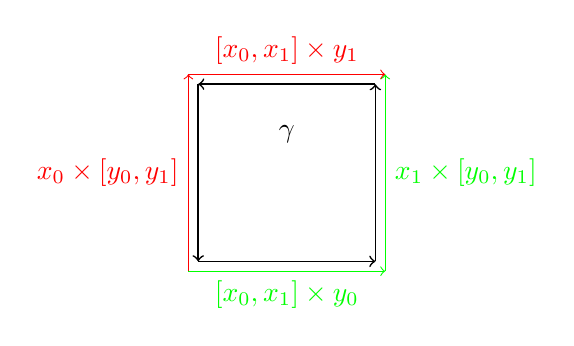
\begin{tikzpicture}[scale=2.5]
        \path[shift={(0.05,0.05)},scale=0.9,semithick]
            (0,0) edge[->] (1,0)
            (1,0) edge[->] (1,1)
            (1,1) edge[->] node[below=4mm] {$\gamma$} (0,1)
            (0,1) edge[->] (0,0);
        \path
            (0,0) edge[->,green] node[anchor=90] {$[x_0,x_1]\times y_0$} (1,0)
            (1,0) edge[->,green] node[anchor=180] {$x_1\times[y_0,y_1]$} (1,1)
            (0,0) edge[->,red] node[anchor=0] {$x_0 \times [y_0,y_1]$} (0,1)
            (0,1) edge[->,red] node[anchor=-90] {$[x_0,x_1] \times y_1$} (1,1);
    \end{tikzpicture}
    \caption{Orientierung der Rechtecks-Randkurve $\gamma$ und der Strecken aus \eqref{eq:winding-number_boundary}}
    \label{fig:rectboundary}
\end{figure}

Im Folgenden seien $\Gamma, \gamma, F$ stets gemäß \ref{thm:def:wn1} definiert.

% fixme: illustration

\begin{proposition}[Subdivision] \label{thm:winding-number_subdivision}
    Sei $(\Gamma_{ij})_{i,j=0}^{n,m}$ eine Unterteilung von $\Gamma$.
    Dann gilt
    \begin{math}
        \deg(F|\Boundary\Gamma) = \sum_{i=1}^n \sum_{j=1}^m \deg(F|\Boundary\Gamma_{i,j}).
    \end{math}
    \begin{proof}
% fixme: illustration
        Betrachte die rechte Seite der Gleichung: die Randterme aus \eqref{eq:winding-number_boundary} heben sich gegenseitig an allen inneren Rändern auf.
        Die restlichen Terme ergeben dank der Subdivisions-Eigenschaft des Cauchy-Index aus \ref{thm:prop:ci_prop} gerade wieder die nötigen Terme für die linke Seite der Gleichung.
    \end{proof}
\end{proposition}

\begin{proposition}[Normierung] \label{thm:prop:wn1_norm}
    Sei $F(z) := z - z_0$ für $z_0 \in \C$.
    Dann gilt
    \begin{math}
        \deg(F|\Boundary\Gamma)
        = \begin{cases}
            1 & \text{falls $z_0 \in \Gamma \setminus \Boundary\Gamma$,} \\
            0 & \text{falls $z_0 \not\in \Gamma$.}
        \end{cases}
    \end{math}
    \begin{proof}
        Falls $z_0 \not\in \Gamma$, dann ist $\Re F(z) \neq 0$ und $\Im F(z) \neq 0$ auf ganz $\Gamma$.
        Alle Terme aus \eqref{eq:winding-number_boundary} verschwinden somit.

        Sei nun $z_0 \in \Gamma \setminus \Boundary\Gamma$.
        Dank der Transformationseigenschaft des Cauchy-Index können wir $z_0 = 0$ und $\Gamma = [-1, 1]\times [-1, 1]$ voraussetzen.
        %fixme: genaue wahl der transformation
        Wir haben dann
        \begin{math}
            \deg(F|\Boundary\Gamma)
            &= \frac{1}{2}\big( \Index{[-1,1]}{x}{-1} + \Index{[-1,1]}{1}{x} - \Index{[-1,1]}{x}{1} - \Index{[-1,1]}{-1}{x} \big) \\
            &= \frac{1}{2}\big( 0 + 1 - 0 - (-1)\big) \\
            &= 1.
        \end{math}
    \end{proof}
\end{proposition}

\begin{lemma} \label{thm:lem:wn1_rot}
    Solange $F(x,y) \neq 0$ in allen Eckpunkten von $\Gamma$ gilt, so ist die Windungszahl invariant unter Drehung um 90°:
    \begin{math}
        \deg(F|\Boundary\Gamma) = \deg(i F|\boundary \Gamma).
    \end{math}
    \begin{proof}
        Sei $\gamma: [0,1] \to \C$ eine Parametrisierung von $\Boundary\Gamma$ wie in \ref{thm:def:wn1}.
        Diese besteht aus vier polynomiellen Stücken und $F\circ \gamma$ besitzt an den Rändern dieser Stücke nach Voraussetzung keine Nullstelle.
        Die Inversionsformel für den Cauchy-Index liefert dann
        \begin{math}
            \deg(F|\Boundary\Gamma) - \deg(iF|\Boundary\Gamma)
            &= \Index{[0,1]}{\Re(F\circ \gamma)}{\Im(F \circ \gamma)} + \Index{[0,1]}{\Im(F\circ\gamma)}{\Re(F\circ\gamma)} \\
            &= \Index{[0,1]}{1}{\Re(F\circ \gamma)\cdot \Im(F\circ \gamma)} \\
            &= 0,
        \end{math}
        da $F \circ \gamma$ geschlossen ist.
    \end{proof}
\end{lemma}

\begin{lemma} \label{thm:lem:winding-number_local}
    Sei $F(x,y) \neq 0$.
    Dann existiert $\delta > 0$, sodass für alle Rechtecke $\tilde \Gamma \subset \Gamma_\delta := [x-\delta, x+\delta] \times [y-\delta, y+\delta]$ gilt
    \begin{math}
        \deg(F|\Boundary\tilde \Gamma) = 0.
    \end{math}
    \begin{proof}
        Dank \ref{thm:lem:wn1_rot} können wir annehmen, dass $\Im F(x,y) \neq 0$.
        Da $F$ stetig ist, existiert $\delta > 0$ sodass $\Im F(x,y) \neq 0$ auf ganz $\Gamma_\delta$.
        Folglich verschwinden alle Terme in $\deg(F|\Boundary\tilde\Gamma)$.
    \end{proof}
\end{lemma}

\begin{lemma} \label{thm:lem:wn1_null}
     Sei $F(x,y) \neq 0$ auf ganz $\Gamma$, dann gilt
     \begin{math}
         \deg(F|\Boundary\Gamma) = 0.
     \end{math}
     \begin{proof}
        $\Gamma$ ist überdeckt von Rechtecken $\Gamma_{\delta(x,y)}$ gemäß \ref{thm:lem:winding-number_local}.
        Da $\Gamma$ kompakt ist, existiert eine \emph{Lebesgue-Zahl} $\lambda > 0$, sodass jedes Quadrat in $\Gamma$ mit Seitenlänge $< \lambda$ jeweils in einem Rechteck $\Gamma_{\delta(x,y)}$ mit $(x,y) \in \Gamma$ enthalten ist.
        Wähle eine Zerlegung gemäß \ref{thm:winding-number_subdivision} mit $n := m := \ceil{\frac{1}{\lambda}}$ und $x_i := y_i := \frac{i}{n}$ für $i = 0, \dotsc, n$.
        Nach \ref{thm:lem:winding-number_local} gilt für jedes $\Gamma_{ij}$ unserer Unterteilung also $\deg(F|\Boundary \Gamma_{ij}) = 0$ und dank Subdivision aus \ref{thm:winding-number_subdivision} $\deg(F|\Boundary\Gamma) = 0$.
     \end{proof}
\end{lemma}

\begin{proposition}[Homotopie-Invarianz]
    Seien $\gamma_0, \gamma_1: [0,1] \to \C^*$ zwei homotope Kurven, d.h. es existiert eine Homotopie $F: [0,1] \times [0,1] \to \C^*$ mit $F(0,t) = \gamma_0(t)$, $F(1,t) = \gamma_1(t)$ und $F(s,0) = F(s,1)$ für alle $s,t \in [0,1]$.

    Dann gilt $\deg(\gamma_0) = \deg(\gamma_1)$.
    \begin{proof}
        Lemma \ref{thm:lem:wn1_null} liefert sofort
        \begin{math}
            0 = \deg(F|\Boundary\Gamma)
            &= \deg(F|_{[0,1]\times 0}) + \deg(\gamma_0) - \deg(F_{[0,1] \times 1}) - \deg(\gamma_1) \\
            &= \deg(\gamma_0) - \deg(\gamma_1).
        \end{math}
    \end{proof}
\end{proposition}


Wir wollen nun die Multiplikativität der Windungszahl in Angriff nehmen.
Seien dazu $\gamma_0 = p + iq$, $\gamma_1 = r + is$ für $p,q,r,s \in \R[x]$ zwei Kurven.
Das Produkt $\gamma_0 \cdot \gamma_1$ ist von der Form
\begin{math}
    \gamma_0 \cdot \gamma_1 = (pr - qs) + (ps + qr)i.
\end{math}
Ähnlich wie uns die Inversionsformel für den Cauchy-Index die Invarianz unter Drehung um 90° (siehe \ref{thm:lem:wn1_rot}) beschert hat, so wird uns eine Produktregel für den Cauchy-Index, welche $\Index{}{pr - qs}{ps + qr}$ mit $\Index{}{p}{q}$ und $\Index{}{r}{s}$ in Beziehung setzt, die Multiplikativität der Windungszahl liefern.

\begin{lemma}[Produktregel des Cauchy-Index] \label{thm:lem:ci_prod}
    Seien $p, q, r, s: \R \to \R$ stückweise polynomielle Funktionen mit $\gamma_0 = p + iq, \gamma_1 = r + is: [a,b] \to \C^*$.
    Dann gilt
    \begin{math}
        \Index{[a,b]}{pr - qs}{ps + qr}
        = \Index{[a,b]}{p}{q} + \Index{[a,b]}{r}{s} - \Index{[a,b]}{1}{qs(ps + qr)}.
    \end{math}
    \begin{note}
        \begin{itemize}
            \item
                Es genügt, vorauszusetzen, dass $\gamma_0, \gamma_1$ an den Rändern der polynomiellen Stücke keine Nulldurchgänge besitzen.
            \item
                Die Produktregel ist eine Verallgemeinerung der Inversionsformel aus \ref{thm:prop:ci_prop}, diese erhält man beispielsweise für $r = 0$ und $s = 1$ (entspricht einer Multiplikation mit $i$ oder eine Drehung um 90°).
        \end{itemize}
    \end{note}
    \begin{proof}
        Betrachte zunächst die einfachen Fälle.
        Für $p = 0$ reduziert sich die Aussage auf $\Index{}{-qs}{qr} = \Index{}{r}{s} - \Index{}{1}{q^2rs}$.
        Wegen $\gamma_0: [a,b] \to \C^*$ muss $q = \const$ sein, d.h. $q^2 > 0$.
        Dank Homogenität ist dies also gerade die Inversionsformel aus \ref{thm:prop:ci_prop}.

        Im Fall $q = 0$ ist $p = \const$ und wir erhalten die Aussage $\Index{}{pr}{ps} = \Index{}{r}{s} - \Index{}{1}{0}$, welche nach Homogenität erfüllt ist.
        Die Fälle $r = 0$ oder $s = 0$ folgen mit der Symmetrie $(p,q,r,s) \mapsto (r,s,p,q)$.

        Dank Subdivision können wir davon ausgehen, dass $p,q,r,s \in \R[x]$ Polynome sind.
        Die Ausdrücke $\Index{}{p}{q}$ und $\Index{}{r}{s}$ liegen bereits gekürzt vor.
        Auch $\Index{}{pr-qs}{ps+qr}$ ist gekürzt, denn angenommen beide Terme verschwinden in $x_0 \in [a,b]$, so ist $q(x_0) \neq 0$ oder $s(x_0) \neq 0$ (sonst müsste $(pr)(x_0) = 0$ und $\Index{}{p}{q}$ oder $\Index{}{r}{s}$ wären nicht gekürzt).
        Sei ohne Einschränkung $q(x_0) \neq 0$, dann gilt
        \begin{math}
            (qs^2)(x_0) = (prs)(x_0) = -(qr^2)(x_0),
        \end{math}
        also $s^2(x_0) = -r^2(x_0)$ und $s(x_0) = r(x_0) = 0$, ein Widerspruch dazu, dass $\Index{}{r}{s}$ bereits gekürzt vorliegt.

        Wir betrachten nun für $x \in [a,b]$ das Intervall $\Gamma_\epsilon(x)$, wobei $\epsilon > 0$ hinreichend klein gewählt ist, dass \ref{thm:lem:wn0_const} für $q$, $s$, $ps + qr$ und $qs(ps + qr)$ erfüllt ist und $p$, $r$, $pr - qs$ auf $\Gamma_\epsilon$ konstant ist.
        Da nur die Nullstellen von $q$, $s$ und $ps + rq$ relevant sind müssen wir dank der Symmetrie $(p,q,r,s) \mapsto (r,s,p,q)$ nur die folgenden Fälle unterscheiden:
        \begin{itemize}
            \item
                Sei $q(x) = 0$ und $s(x) \neq 0$.
                In diesem Fall ist $ps+rq(x) \neq 0$.
                Durch die Symmetrie $(q,s) \mapsto (-q,-s)$ können wir Annehmen, dass $ps + rq > 0$ gilt und somit auch $ps > 0$.
                Wir erhalten
                \begin{math}
                    \Index{}{p}{q} + \Index{}{r}{s} - \Index{}{1}{qs(ps+qr)}
                    = \Index{}{ps}{qs} - \Index{}{1}{qs}
                    = 0
                    = \Index{}{pr-qs}{ps+qr}.
                \end{math}
            \item
                Sei $q(x) \neq 0 \neq s(x)$, aber $(ps + qr)(x) = 0$.
                Angenommen $(pr - qs)(x) = 0$, dann ist
                \begin{math}
                    (qs^2)(x)
                    = (prs)(x)
                    = -(qr^2)(x),
                \end{math}
                d.h. $s^2(x) = -r^2(x)$ und somit $s(x) = 0$, ein Widerspruch.
                Also ist $(pr - qs)(x) \neq 0$ und $\Index{}{pr-\nobreak qs}{ps+qr}$ liegt in gekürzter Form vor.
                Wegen $(ps + rq)(x) = 0$ können wir den vorderen Term im Cauchy-Index abändern:
                \begin{math}
                    \Index{}{pr-qs}{ps+qr}
                    &= \Index{}{prqs - q^2s^2}{qs(ps+qr)} \\
                    &= \Index{}{-p^2s^2 -q^2s^2}{qs(ps+qr)} \\
                    &= -\Index{}{(p^2 + q^2)s^2}{qs(ps+qr)}
                    = -\Index{}{1}{qs(ps+qr)}.
                \end{math}
                Beachte, dass durch die Umformungen keine neuen Nullstellen in $x$ im ersten Argument des Cauchy-Index eingeführt wurden, alle Ausdrücke liegen also in gekürzter Form vor.

                Wegen $\Index{}{p}{q} = \Index{}{r}{s} = 0$ ist also der Fall erledigt.
            \item
                Sei $q(x) = s(x) = 0$, also auch $(ps + qr)(x) = 0$.
                Durch Subdivision und Antisymmetrie können wir davon ausgehen, dass $\Gamma_\epsilon(x)$ von der Form $[x, x + \epsilon]$ ist.
                Auswertungen von $q$, $s$ und $ps + qr$ in $x$ verschwinden und $p$, $r$ und $pr - qs$ besitzen auf $\Gamma_\epsilon(x)$ konstantes Vorzeichen ungleich Null.

                Unter Verwendung der abkürzenden Notation $\sgn(p) := \sgn(p(x+\epsilon))$ reduziert sich also die Behauptung auf
                \begin{math}
                    \sgn(pr)\sgn(ps+qr)
                    = \sgn(pq) + \sgn(rs) - \sgn(qs)\sgn(ps+qr).
                \end{math}
                Mittels der Symmetrie $(q,s) \mapsto (-q,-s)$ können wir von $\sgn(ps + qr) = 1$ ausgehen und erhalten nach Umformung
                \begin{math}
                    \big(\sgn(p) - \sgn(s)\big)\big(\sgn(r) - \sgn(q)\big) = 0.
                \end{math}
                Dies ist jedoch aufgrund der jüngsten Annahme $\sgn(ps + qr) = 1$ erfüllt, denn $ps > 0$ oder $qr > 0$.
        \end{itemize}
    \end{proof}
\end{lemma}

\begin{corollary}[Multiplikativität] \label{thm:cor:wn1_mult}
    Seien $\gamma_0, \gamma_1: [a,b] \to \C^*$ stückweise polynomielle, geschlossene Kurven.
    Dann gilt
    \begin{math}
        \deg(\gamma_0 \cdot \gamma_1) = \deg(\gamma_0) + \deg(\gamma_1).
    \end{math}
    \begin{proof}
        Dies folgt im Wesentlichen aus \ref{thm:lem:ci_prod} mittels $\gamma_0 = p + iq$, $\gamma_1 = r + is$, also $\gamma_0\cdot\gamma_1 = (pr-qs) + (ps +qr)i$.
        Der Term $\Index{}{1}{qs(ps+qr)}$ entfällt, da die Kurven geschlossen sind:
        \begin{math}
            \Index{}{1}{qs(ps+qr)}
            = \frac{1}{2}\Big(\sgn\big(qs(ps+qr)\big)(b) - \sgn\big(qs(ps+qr)\big)(a)\Big)
            = 0.
        \end{math}
    \end{proof}
\end{corollary}

\begin{corollary}[Zählen komplexer Nullstellen] \label{thm:cor:complex-roots}
    Sei $F \in \C[z]$ ein komplexes Polynom und $\Gamma := [x_0,x_1] \times [y_0, y_1] \subset \C$ ein Rechteck sodass $F(z) \neq 0$ auf $\Boundary\Gamma$.
    Dann zählt $\deg(F|\Boundary\Gamma)$ die Anzahl der komplexen Nullstellen von $F$ auf $\Gamma$.
    \begin{proof}
        Wir faktorisieren $F = (z-z_0)(z-z_1) \dotsb(z-z_m) G$, sodass $G$ keine Nullstellen auf $\Gamma$ besitzt.
        Die Multiplikativität aus \ref{thm:cor:wn1_mult} liefert
        \begin{math}
            \deg(F|\Boundary\Gamma) = \underbrace{\deg(z-z_0|\Boundary\Gamma)}_{=1} + \dotsb + \underbrace{\deg(z-z_m|\Boundary\Gamma)}_{=1} + \underbrace{\deg(G|\Boundary\Gamma)}_{=0},
        \end{math}
        dank \ref{thm:prop:wn1_norm} und \ref{thm:lem:wn1_null}.
    \end{proof}
    \begin{note}
        \begin{itemize}
            \item
                Es genügt vorauszusetzen, dass $F(z) \neq 0$ in den Ecken des Rechtecks $\Gamma$ gilt (siehe Bemerkung zur Produktformel).
                Nullstellen auf dem Rand des Rechtecks werden dann mit dem Faktor $\frac{1}{2}$ gezählt.
            \item
                Im Gegensatz zu \ref{thm:prop:ci_roots_multiple} werden hier die Nullstellen mitsamt ihrer Vielfachheit gezählt.
        \end{itemize}
    \end{note}
\end{corollary}

\begin{remark}[Lokalisieren von Nullstellen]
    Die Resultate aus \ref{thm:cor:complex-roots} und \ref{thm:alg:ci_premseq} stellen zusammen nicht nur einen Algorithmus bereit, um die Anzahl der komplexen Nullstellen eines Polynoms innerhalb eines Rechtecks zu zählen.
    Wir können sie auch zum lokalisieren und approximieren aller Nullstellen eines Polynoms einsetzen.

    Sei $F \in \C[z]$ ein komplexes Polynom.
    Man starte mit einem hinreichend großen Rechteck $\Gamma$, welches alle Nullstellen von $F$ enthält (man nutze dazu eine entsprechende Abschätzung wie beispielsweise in \cite[Proposition 5.8]{eisermann2012fundamental}).
    Dieses teilt man in vier kleinere Rechtecke gleicher Größe und berechnet die Anzahl Nullstellen von $F$ innerhalb dieser Rechtecke.
    Rechtecke ohne Nullstellen werden verworfen und der Prozess mit den verbleibenden Rechtecken iteriert.
    Nach endlich vielen Schritten hat man nun Rechtecke gefunden, die jeweils höchstens eine Nullstelle enthalten.

    Beachte, dass Nullstellen in den Ecken der Rechtecke einzelnd geprüft und herausdividiert werden können.
    Nullstellen an den Kanten der Rechtecke werden mit der Gewichtung $\frac{1}{2}$ gezählt.

    Nach einer groben Lokalisierung mit obigem Verfahren kann man die Nullstellen anschließend beispielsweise mit einem Newton-Verfahren schneller approximieren.

    Details und Aussagen zur Komplexität eines solchen Algorithmus finden sich in \cite[§6.3~--~§6.10]{eisermann2012fundamental}.
\end{remark}








%\begin{tikzpicture}
%    \begin{axis}
%        \addplot3[surf,faceted color=black,color=red,colormap/greenyellow]({x},{y},{x^2});
%    \end{axis}
%\end{tikzpicture}



\clearpage

\chapter{Der bivariate Fall: Abbildungsgrad und Kronecker-Index} \label{sec:2}


\section{Geometrische Motivation}


Im Kapitel \ref{sec:1} haben wir die Windungszahl anhand des Cauchy-Index definiert:
\begin{math}
    \deg(\gamma) = \frac{1}{2} \Index{[a,b]}{\Re \gamma}{\Im \gamma}.
\end{math}
Unser nächster Schritt ist eine Verallgemeinerung der Windungszahl eine Dimension höher: der \emph{Abbildungsgrad}.

Sei $\S^n$ für $n \in \N$ die $n$-dimensionale Sphäre.
Der Abbildungsgrad ordnet jeder stetigen Abbildung $\phi: \S^n \to \S^n$ eine Zahl $\deg(\phi) \in \Z$ zu, welche anschaulich die (orientierte) Anzahl Wicklungen der Sphäre um sich selbst zählt.
Für eine Illustration siehe Abbildung \ref{fig:spherewinding}.

\begin{figure}[ht]
    \centering
    \begin{tikzpicture}[baseline=(current bounding box.center)]
        \begin{axis}[
            scale=2,
            view={115}{30},
            unit vector ratio={1 1 1},
            %xmin=-1.2,xmax=1.2,
            %ymin=-1.2,ymax=1.2,
            %zmin=-1,zmax=1.5,
            %axis lines=center,
            %axis x line=none,
            %axis y line=center,
            %axis z line=center,
            hide axis,
        ]
        %\draw[-] (axis cs:-2,0,0) -- (axis cs:1,0,0);
        \addplot3[
            raw gnuplot,
            parametric,
            surf,
            z buffer=sort,
            %shader=flat,
            %mesh/interior colormap={blueblack}{color=(black) color=(blue)},
            %mesh/interior colormap name=greenyellow2,
            %colormap name=greenyellow,
        ] gnuplot {
            set parametric;
            set hidden3d;
            set isosamples 40,10;
            set urange [-2*pi:2*pi];
            set vrange [0:pi/2];
            splot -((u+pi)/(9*pi) + 1)*sin(v)*cos(u/2),-((u+pi)/(9*pi)+1)*sin(v)*sin(u/2),-cos(v)
        };
        %\draw[-stealth] (axis cs:1,0,0) -- (axis cs:2,0,0);
        \addplot3[
            raw gnuplot,
            parametric,
            surf,
            %z buffer=sort,
            z buffer=reverse y seq,
            %shader=flat,
            %mesh/interior colormap={blueblack}{color=(black) color=(blue)},
            %mesh/interior colormap name=greenyellow2,
            %colormap name=greenyellow,
        ] gnuplot {
            set parametric;
            set hidden3d;
            set isosamples 40,10;
            set urange [-2*pi:2*pi];
            set vrange [0:pi/2];
            splot -((u+pi)/(9*pi) + 1)*sin(v)*cos(u/2),-((u+pi)/(9*pi)+1)*sin(v)*sin(u/2),cos(v) + 0.3
        };
        \end{axis}
    \end{tikzpicture}
    \quad
    \begin{tikzpicture}[baseline=(current bounding box.center)]
        \begin{axis}[
            scale=2,
            view={115}{30},
            unit vector ratio={1 1 1},
            %xmin=-1.2,xmax=1.2,
            %ymin=-1.2,ymax=1.2,
            %zmin=-1,zmax=1.5,
            %axis lines=center,
            %axis x line=none,
            %axis y line=center,
            %axis z line=center,
            hide axis,
        ]
        %\draw[-] (axis cs:-2,0,0) -- (axis cs:1,0,0);
        \addplot3[
            raw gnuplot,
            parametric,
            surf,
            z buffer=sort,
            %shader=flat,
            %mesh/interior colormap={blueblack}{color=(black) color=(blue)},
            %mesh/interior colormap name=greenyellow2,
            %colormap name=greenyellow,
        ] gnuplot {
            set parametric;
            set hidden3d;
            set isosamples 80,10;
            set urange [-2*pi:2*pi];
            set vrange [0:pi/2];
            splot ((u+pi)/(9*pi) + 1)*sin(v)*cos(u),((u+pi)/(9*pi)+1)*sin(v)*sin(u),-cos(v)
        };
        %\draw[-stealth] (axis cs:1,0,0) -- (axis cs:2,0,0);
        \addplot3[
            raw gnuplot,
            parametric,
            surf,
            %z buffer=sort,
            z buffer=reverse y seq,
            %shader=flat,
            %mesh/interior colormap={blueblack}{color=(black) color=(blue)},
            %mesh/interior colormap name=greenyellow2,
            %colormap name=greenyellow,
        ] gnuplot {
            set parametric;
            set hidden3d;
            set isosamples 80,10;
            set urange [-2*pi:2*pi];
            set vrange [0:pi/2];
            splot ((u+pi)/(9*pi) + 1)*sin(v)*cos(u),((u+pi)/(9*pi)+1)*sin(v)*sin(u),cos(v) + 0.3
        };
        \end{axis}
    \end{tikzpicture}
    \caption{Einfache und zweifache Wicklung der Sphäre $\S^2$, zur Vergleichbarkeit jeweils horizontal aufgeschnitten und vertikal aufgefächert}
    \label{fig:spherewinding}
\end{figure}

Im univariaten Fall für $n = 1$ haben wir die Windungszahl für eine stückweise polynomielle, geschlossene Kurve $\gamma: [0,1] \to \C^*$ definiert.
Wir können $\gamma$ auch als Abbildung $\phi: \S^1 \to \S^1$ betrachten, z.B. über $\phi(e^{2\pi i t}) := \frac{\gamma(t)}{|\gamma(t)|}$.
Auf die Weise wird dank $\gamma(0) = \gamma(1)$ der Parameterbereich $[0,1]$ durch $\S^1$ ersetzt, während im Bildbereich radial auf $\S^1$ projiziert wird.

Versuchen wir dies bivariat zu verallgemeinern, so ist zunächst nicht eindeutig, was für eine auf einem Rechteck $\Gamma$ parametrisieren Fläche $f: \Gamma \to \R^3 \setminus \Set 0$ die Eigenschaft „geschlossen“ bedeuten soll: es bieten sich verschiedene Möglichkeiten an, die Ränder von $\Gamma$ unter $f$ so zu identifizieren, dass eine gewisse Periodizität entsteht.
Wir können dieser Überlegung aus dem Weg gehen, indem wir die Sphäre $\S^2$ im Parameterbereich durch den Rand eines Kubus ersetzen (beispielsweise über $x \mapsto \frac{x}{\|x\|_\infty}$).
Dieser Kubusrand kann nun in seine sechs Seitenflächen zerlegt werden, welchen wir einzelnd einen Abbildungsgrad zuordnen werden.
Die gleiche Überlegung fand bereits im Abschnitt \ref{sec:wn_geom} statt, als wir die vier Randseiten eines Rechtecks betrachtet haben, siehe auch Abbildung \ref{fig:cube-boundary}.

Wir werden uns für ein Rechteck $\Gamma = [x_0,x_1] \times [y_0,y_1]$ stückweise polynomielle Flächen $f = (p,q,r): \Gamma \to \R^3 \setminus \Set 0$ anschauen und versuchen einen Index $\Index{\Gamma}{p}{q,r}$ als Analogon zum Cauchy-Index zu finden.

Während wir im univariaten Fall die Schnittpunkte von $\gamma$ mit der reellen Achse analysiert haben, betrachten wir nun die Schnittpunkte von $f$ mit der $e_0$-Achse, d.h. diejenigen Punkte, an denen die Koordinatenfunktionen $q$ und $r$ Null ergeben.
Solche Punkte bezeichnen wir dank der geometrischen Anschauung auch als \emphdef{Durchstoßpunkte}.

Wir wollen die Zählung dieser Punkte analog zum ersten Kapitel motivieren.
Dazu betrachten wir Abbildung \ref{fig:idx_counting}.
Im univariaten Fall hat das Vorzeichen von $p$ und die Art des Vorzeichenwechsels von $q$ die Zählung bestimmt, während hier das Vorzeichen von $p$ und die Orientierung der Fläche (bestimmt durch $q, r$) an der jeweiligen Stelle maßgebend sind.

Um die Orientierung der Fläche (bezüglich der $e_0$-Achse) an einem Durchstoßpunkt zu erhalten, können wir die Windungszahl aus dem ersten Kapitel nutzen.
Dazu betrachten wir, wie $(q, r): \R^2 \to \R^2$ ein kleines Rechteck $\Gamma_\epsilon(x,y)$ um die Durchstoßstelle $(x,y) \in \R^2$ abbildet.
Die Windungszahl vom Rand des Bild-Rechtecks $\deg\big((q,r)|\Boundary\Gamma_\epsilon(x,y)\big)$ liefert die Orientierung der Fläche an dieser Stelle (sofern das Rechteck nicht mehrfach gewindet wurde, mehr dazu später).
Geometrisch betrachtet projizieren wir also das Flächenstück auf die $e_1,e_2$-Ebene und werten dort die Windungszahl aus.

Zusammen mit dem Vorzeichen von $p$ ergibt sich für die Zählung dieses Durchstoßpunktes:
\begin{math}
    \Index{\Gamma_\epsilon(x,y)}{p}{q,r}
    = \sgn(p(x,y)) \deg\big((q,r)|\Boundary\Gamma_\epsilon\big).
\end{math}
Diese Form kommt uns bekannt vor: in der Tat bildet sie das Analogon zur Definition des lokalen Cauchy-Index aus \ref{thm:def:ci}.
Statt $\deg\big((q,r)|\Boundary\Gamma_\epsilon\big)$ werden wir im Folgenden verkürzt $\deg(q,r|\Boundary\Gamma_\epsilon)$ schreiben.
Die Summe von $\Index{\Gamma_\epsilon(x,y)}{p}{q,r}$ über alle Durchstoßpunkte bezeichnen wir als \emphdef{Kronecker-Index} und schreiben $\Index{\Gamma}{p}{q,r}$.

Global betrachtet fällt auf, dass wir mit dieser Zählung genau wie im ersten Kapitel den doppelten Abbildungsgrad erhalten (gezählt wird auf beiden Seiten der $e_0$-Achse).
Dies motiviert
\begin{math}
    \deg(f) = \frac{1}{2} \Index{\Gamma}{p}{q,r}.
\end{math}


\section{Der Kronecker-Index}

Wir werden nun einige Vorkehrungen treffen, um die Art der Durchstoßstellen besser kontrollieren zu können und eine saubere Definition des Index zu ermöglichen.

%Der bivariate Fall beherbergt allerdings wesentliche Tücken, die wir nur teilweise in den Griff bekommen werden.
%Es wird versucht, jede nötige Einschränkung kurz zu begründen.


\begin{definition}
    Seien $q, r \in \R[x,y]$ und $\Gamma := [x_0, x_1] \times [y_0, y_1]$.
    Wir definieren die gemeinsame Nullstellenmenge von $q, r$ auf $\Gamma$ als
    \begin{math}
        V_\Gamma(q,r) :=
        \Set{(x,y) \in \Gamma & q(x,y) = r(x,y) = 0}.
    \end{math}
    Für $p, q, r \in \R[x,y]$ schreiben wir
    \begin{math}
        \_V := \_V(p,q,r) := V(p,q) \cup V(q,r) \cup V(r,p).
    \end{math}
    Wenn $p, q, r$ aus dem Kontext klar sind, schreiben wir auch $\_V_\Gamma$ oder nur $\_V$.
\end{definition}

$V_\Gamma$ hat idealerweise die Gestalt wie in Abbildung ??, kann jedoch auch nicht-isolierte Punkte enthalten, wenn beispielsweise $q$ und $r$ gleiche Faktoren besitzen.

\begin{definition}
    Seien $p, q, r \in \R[x]$, $\Gamma := [x_0, x_1] \times [y_0, y_1]$.
    Wir nennen das Tupel $(\Gamma, p, q, r)$ \emphdef{zulässig}, falls
    \begin{enumerate}[i)]
        \item
            $\_V$ diskret ist,
        \item
            $\_V \cap \Boundary \Gamma = \emptyset$ und
        \item
            $p^2 + q^2 + r^2 > 0$ auf $\Gamma$.
    \end{enumerate}
\end{definition}

\begin{definition} \label{thm:def:idx}
    Sei $(\Gamma, p, q, r)$ zulässig.
    Für $(x_0, y_0) \in V_\Gamma$ existiert $\eps > 0$, sodass $p(x,y) \neq 0$ auf $\Gamma_\eps(x_0, y_0)$ und $\Gamma_\eps(x_0, y_0) \cap V = \Set{(x_0, y_0)}$.
    Setze
    \begin{math}
        \Index{(x_0,y_0)}{p}{q,r} &:= \sgn(p) \deg(q,r|\Boundary\Gamma_\eps), \\
        \Index{\Gamma}{p}{q,r} &:= \sum_{(x_0,y_0) \in V_\Gamma} \Index{(x_0,y_0)}{p}{q,r}.
    \end{math}
    Wir nennen $\Index{\Gamma}{p}{q,r}$ \emphdef{Kronecker-Index} von $p, q, r$ auf $\Gamma$.
\end{definition}

\begin{note}
    Die Idee eines solchen Index $\Index{\Gamma}{p}{q,r}$ geht auf die sogenannte „Charakteristikentheorie“ von Kronecker zurück, wie sie z.B. im Lehrbuch von Weber \cite[§93-95]{weber1895lehrbuch} zu finden ist.

    Dazu werden die Nullstellenmengen $p = 0$, $q = 0$, $r = 0$ als geschlossene Kurven auf einem beschränktem Gebiet betrachtet.
    Schnittpunkte eines Paares von Kurven werden nun mit Hilfe der dritten Kurve auf orientierte Weise gezählt (genaueres in \cite[§94]{weber1895lehrbuch}).

    Ein wesentlicher Unterschied zwischen Kroneckers Charakteristik und unserem Index besteht darin, dass Kronecker die globale Nullstellenmengen betrachtet, während wir uns auf ein beliebiges Rechteck $\Gamma$ beschränken können.
    Dies spiegelt sich auch darin wieder, dass Kronecker im Gegensatz zu uns seine Charakteristik bereits mit dem Faktor $\frac{1}{2}$ versieht, was dem Abbildungsgrad gleich käme und allgemein nur ganzzahlig möglich ist, wenn global gezählt wird.

    Durch diese globale Betrachtungsweise bleibt Kroneckers Charakteristik invariant unter zyklischer Permutation aller $p, q, r$.
\end{note}

\section{Eigenschaften}

\begin{proposition}[Eigenschaften] \label{thm:prop:idx_prop}
    Seien $(\Gamma, p, q, r)$ zulässig.
    Der Kronecker-Index genügt folgenden Eigenschaften:
    \begin{enumerate}[i)]
        \item
            \emph{Subdivision}: Für $V_{\Gamma_1} \cup V_{\Gamma_2} = V_\Gamma$, $V_{\Gamma_1} \cap V_{\Gamma_2} = \emptyset$ gilt
            \begin{math}
                \Index{\Gamma}{p}{q,r} = \Index{\Gamma_1}{p}{q,r} + \Index{\Gamma_2}{p}{q,r},
            \end{math}
        \item
            \emph{Homogenität}: Falls $\sgn(s) = \const \neq 0$ auf ganz $\_V$ und $s(x,y) \neq 0$ auf $\Boundary\Gamma$, so gilt
            \begin{math}
                \sgn(s) \Index{\Gamma}{p}{q,r}
                = \Index{\Gamma}{sp}{q,r}
                = \Index{\Gamma}{p}{sq,r}
                = \Index{\Gamma}{p}{q,sr}.
            \end{math}
        \item
            \emph{Scherung}:
            $
                \Index{\Gamma}{p}{q,r} = \Index{\Gamma}{p+s_1q + s_2r}{q,r}.
            $
        \item
            \emph{Antikommutativität}:
            $
                \Index{\Gamma}{p}{q,r} = - \Index{\Gamma}{p}{r,q}.
            $
        \item
            \emph{Inversion}: Es gilt
            \begin{math}
                \Index{\Gamma}{p}{q,r} + \Index{\Gamma}{q}{p,r} &= \Index{\Gamma}{1}{pq,r}, \\
                \Index{\Gamma}{p}{q,r} + \Index{\Gamma}{r}{q,p} &= \Index{\Gamma}{1}{q,pr}.
            \end{math}
        \item
            \emph{Reduktion}:
            $
                \Index{\Gamma}{1}{q,r} = \deg(q,r|\Boundary\Gamma).
            $
    \end{enumerate}
    \begin{proof}
        \begin{enumerate}[i)]
            \item
                Da $V_\Gamma, V_{\Gamma_1}, V_{\Gamma_2}$ ausschließlich aus isolierten Punkten besteht lässt sich $\eps$ in der Definition \ref{thm:def:idx} hinreichend klein wählen, dass alle $\Gamma_\eps(x,y)$ für $(x,y) \in V_\Gamma$ disjunkt sind.

                Da $V_\Gamma$ die disjunkte Vereinigung von $V_{\Gamma_1}, V_{\Gamma_2}$ ist, folgt die Aussage aus der Summation in \ref{thm:def:idx}.
            \item
                Zunächst ist $V(q,r) = V(sq,r) = V(q,sr)$.
                An jeder Nullstelle $(x,y) \in V$ gilt
                \begin{math}
                    \sgn(s) \Index{\Gamma}{p}{q,r}
                    = \sgn(s) \sgn(p) \deg((q,r)|\Boundary \Gamma_\eps)
                    = \Index{\Gamma}{sp}{q,r}.
                \end{math}
                Außerdem ist
                \begin{math}
                    \sgn(s) \Index{\Gamma}{p}{q,r}
                    = \sgn(p) \sgn(s)\deg((q,r)|\Boundary \Gamma_\eps)
                    = \sgn(p) \deg((sq,r)|\Boundary \Gamma_\eps)
                    = \Index{\Gamma}{sp}{q,r},
                \end{math}
                da $\deg(\argdot)$ die Homogenität des Cauchy-Index erbt.
                Der letzte Fall verläuft analog.
            \item
                In jedem Punkt $(x,y) \in V$ ist $\sgn(p) = \sgn(p + s_1q + s_2r)$ und die Behauptung folgt.
            \item
                Folgt aus der Invarianz der Windungszahl unter Drehung um 90°, siehe \ref{thm:lem:wn1_rot}.
            \item
                Da $(\Gamma, p, q, r)$ und $(\Gamma, q, p, r)$ zulässig sind, muss $V(q,r) \cap V(p,r) = \emptyset$ gelten.
                Wir können also durch Subdivision davon ausgehen, dass ohne Einschränkung $V(p,r) = \emptyset$.
                Da $p(x,y) \neq 0$ für alle $(x,y) \in V(q,r)$, gilt $V(q,r) = V(pq,r)$.
                Sei also $(x,y) \in V(pq,r)$, dann gilt
                \begin{math}
                    \Index{\Gamma_\epsilon(x,y)}{p}{q,r}
                    &= \sgn(p) \deg(q,r |\Boundary\Gamma_\eps(x,y)) \\
                    &= \deg(pq,r |\Boundary \Gamma_\eps(x,y))
                    = \Index{\Gamma_\epsilon(x,y)}{1}{pq,r}.
                \end{math}
                Die zweite Aussage $\Index{\Gamma}{p}{q,r} + \Index{\Gamma}{r}{q,p} = \Index{\Gamma}{1}{q,pr}$ folgt mit Antikommutativität aus iv).
            \item
                Sei $(x,y) \in V$, dann gilt per definitionem
                \begin{math}
                    \Index{\Gamma_\epsilon(x,y)}{1}{q,r} = \deg(F|\Boundary\Gamma_\eps(x,y)).
                \end{math}
                Dank Subdivision des Kronecker-Index in i) und Subdivision der Windungszahl gemäß \ref{thm:winding-number_subdivision}, sowie \ref{thm:lem:wn1_null} folgt die Aussage durch Summation.
        \end{enumerate}
    \end{proof}
\end{proposition}


\section{Algorithmus}

Beim Cauchy-Index hatten uns die Eigenschaften Scherung, Inversion und Reduktion bereits im Wesentlichen einen Algorithmus zur Berechnung beschert.
Dies war möglich, weil wir den Grad der Polynome mit Hilfe der Scherung und der Inversion reduzieren (beispielsweise über Polynomdivision wie im euklidischen Algorithmus) und die Reduktion auf die verbleibenden Terme anwenden konnten.

Im bivariaten Fall stellen wir zunächst fest, dass wir mit Hilfe der Inversionsformel die Reihenfolge der auftretenden Polynome in $\Index{}{p}{q,r}$ beliebig vertauschen können.
Die dabei auftretenden Inversionsterme der Form $\Index{}{1}{\dotsc}$ lassen sich dank der Reduktion mit den Werkzeugen aus dem ersten Kapitel berechnen.
Wir bezeichnen dieses Vorgehen im Folgenden als \emphdef{Permutieren}.

Es ist im bivariaten Fall mit zwei Variablen allerdings zunächst nicht klar, wie der „Grad eines Polynoms“ zu definieren ist und auf welche Weise wir ihn zuverlässig reduzieren.
Betrachte beispielswiese $p = x^2$, $q = xy$, $r = y^2 \in \R[x,y]$: es besteht keine Hoffnung wie im univariaten Fall alle Variablen in einem Term allein durch Scherung und Permutieren zu eliminieren.

Um diesem Problem entgegenzutreten betrachten wir die Polynome zunächst als Elemente aus $\R[x][y]$, bzw. $\R[y][x]$, d.h. als Polynome in einer Variablen $y$ oder $x$ mit Koeffizienten aus dem Polynomring $\R[x]$, bzw. $\R[y]$.

\begin{definition}
    Sei $p \in \R[x,y]$.
    Wir bezeichnen mit $\deg_x(p)$, $\deg_y(p)$ den Grad des Polynoms $p$ als Element des Polynomrings $\R[y][x]$, bzw $\R[x][y]$ und mit $\lc_x(p) \in \R[y]$, $\lc_y(p) \in \R[x]$ den jeweils führenden Koeffizienten (engl. “leading coefficient”).
\end{definition}


Wir werden die sogenannte pseudo-euklidische Division als Verallgemeinerung der euklidisichen Division nutzen, um in diesen Polynomringen eine Reduzierung einer dieser Grade zu ermöglichen.
Ganz problemfrei ist diese Verallgemeinerung allerdings nicht.

\begin{proposition}[pseudo-euklidische Division] \label{thm:prop:pseucl}
    Sei $R$ ein Integritätsbereich und $p, q \in R[x]$, $q \neq 0$.
    Dann existieren $c \in R$, $s, r \in R[x]$ mit $c \neq 0$, sodass
    \begin{math}
        c p &= s q + r &
        &\text{und}&
        \deg(r) &< \deg(q).
    \end{math}
    Wir nennen $r$ \emphdef{pseudo-euklidischer Rest}.
    \begin{proof}
        Siehe \ref{thm:alg:pseucl}.
    \end{proof}
    \begin{note}
        Der wesentliche Unterschied zur gewöhnlichen euklidischen Division über einem Körper besteht in der Multiplikation von $p$ mit einem Koeffizienten $c \in R$.
    \end{note}
\end{proposition}

\begin{algorithm}[pseudo-euklidische Division] \label{thm:alg:pseucl}
    \Input{$p,q \in R[x]$, $q \neq 0$}\\
    \Output{$c \in R$, $s, r \in R[x]$ sodass $cp = sq + r$ und $\deg(r) < \deg(q)$}
    \begin{algorithmic}[1]
        \State{$(c, s) \gets (1, 0)$}
        \While{$\deg(p) \ge \deg(q)$}
            \State{$c \gets \lc(q) \cdot c$}
            \State{$s \gets \lc(q) \cdot s + \lc(p) \cdot x^{\deg(p) - \deg(q)}$}
            \State{$p \gets \lc(q) \cdot p - \lc(p) \cdot q \cdot x^{\deg(p) - \deg(q)}$}
        \EndWhile
        \State{$r \gets p$}
        \Return{$c, s, r$}
    \end{algorithmic}
    Dabei bezeichnen $\lc(p), \lc(q) \in R$ die Leitkoeffizienten von $p$, bzw. $q$.
    \begin{proof}
        Falls $\deg(p) \ge \deg(q)$, so ist leicht einzusehen, dass jede Iteration den Grad von $p$ in Zeile 5 um mindestens $1$ reduziert, denn das Leitmonom wird eliminiert.
        Der Algorithmus terminiert also nach endlich vielen Schritten.

        Sei $\hat p$ das Polynom $p$ zu Beginn des Algorithmus.
        Zu diesem Zeitpunkt erfüllt $p$ die Gleichung $c\hat p = sq + p$ trivialerweise mit $c = 1$ und $s = 0$.

        Es erfülle nun $p$ zu Beginn eines Iterationsschrittes (unmittelbar vor Zeile 3) die Gleichung $c \hat p = sq + p$ für ein $c \in R$ und $s \in R[x]$.
        Nach der Elimination in Zeile 5 ergibt sich die Form
        \begin{math}
            \tilde p &= \lc(q) p - \lc(p) q x^{\deg(p) - \deg(q)} \\
            &= \lc(q)(c\hat p - sq) - \lc(p) q x^{\deg(p) - \deg(q)} \\
            &= \underbrace{\lc(q)c}_{=\tilde c} \hat p - \underbrace{\big( \lc(q) s + \lc(p) x^{\deg(p)-\deg(q)} \big)}_{=\tilde s} q.
        \end{math}
        Es gilt $\tilde c \in R$, $\tilde s \in R[x]$ und $\tilde c \hat p = \tilde s q + \tilde p$.

        Induktiv erfüllt $p$ also in jedem Schritt die gewünschte Darstellung $c \hat p = sq + p$.
        Bei Abbruch der Schleife gilt zusätzlich notwendigerweise $\deg(p) < \deg(q)$ und der Algorithmus liefert ein korrektes Ergebnis.
    \end{proof}
\end{algorithm}


Betrachten wir jetzt wieder den Kronecker-Index $\Index{\Gamma}{p}{q,r}$ und ermitteln zu $p,q \in \R[x,y] = \R[x][y]$ mit Hilfe von \ref{thm:alg:pseucl} die Darstellung $c p = sq + \tilde p$, wobei $\tilde p$ der pseudo-euklidische Rest sei.
Es ist zu beachten, dass $c$ ein Element aus dem Koeffizientenring ist, d.h. $c \in \R[x]$ ist selbst ein Polynom in einer Variablen.

Falls $\sgn(c) = \const \neq 0$ auf $\_V \cup \Boundary\Gamma$, so gilt für den Kronecker-Index dann mit Homogenität und Scherung
\begin{math}[numbered] \label{eq:idx_prem}
    \Index{}{p}{q, r}
    = \Index{}{cp}{q, r}
    = \Index{}{sq + \tilde p}{q, r}
    = \Index{}{\tilde p}{q, r}
\end{math}
Zusammen mit der Inversionsformel können wir also beispielsweise den $y$-Grad der auftretenden Polynome reduzieren.
Die wichtige Frage für eine korrekte Durchführung lautet nun: „Wann gilt $\sgn(c) = \const \neq 0$ auf $\_V \cup \Boundary\Gamma$?“

Wir können auf einfachem Wege zumindest $c(x) \ge 0$ erreichen.

\begin{corollary} \label{thm:cor:pseucl}
    Seien $p, q \in \R[x,y]$, dann existieren $c \in \R[x]$, $s, r \in \R[x,y]$ mit $c \neq 0$ und $c(x) \ge 0$ auf $\R$, sodass
    \begin{math}
        c p &= s q + r &
        &\text{und}&
        \deg_y(r) &< \deg_y(q).
    \end{math}
    Wir schreiben kurz $\rem_y(p, q) := r$ für einen solchen Rest $r$.

    Analog $\rem_x(p, q) := r$, wenn wir $c \in \R[y]$ und $\deg_x(r) < \deg_x(q)$ fordern.
    \begin{proof}
        Wir betrachten $\R[x,y]$ als Polynomring $\R[x][y]$, bzw. $\R[y][x]$.
        Aus \ref{thm:prop:pseucl} folgt eine Darstellung $\tilde c p = \tilde sq + \tilde r$.
        Die Wahl $c := \tilde c^2$, $s := \tilde c \tilde s$, $r := \tilde c \tilde r$ erfüllt die gewünschten Eigenschaften.
    \end{proof}
    \begin{note}
        Die Terme $c, s$ und $r = \rem(p,q)$ lassen sich also direkt aus dem Ergebnis von \ref{thm:alg:pseucl} ermitteln.
    \end{note}
\end{corollary}

Unter der zugegeben optimistischen Haltung, dass uns die Nullstellen $c(x) = 0$ keine Schwierigkeiten bereiten, können wir nun einen Algorithmus skizzieren, der den Kronecker-Index $\Index{\Gamma}{p}{q,r}$ berechnet.

\begin{algorithm} \label{thm:alg:idx}
    \Input{$p, q, r \in \R[x,y]$ und ein Rechteck $\Gamma \subset \R^2$, wobei $(\Gamma, p, q, r)$ zulässig sei} \\
    \Output{$\Index{\Gamma}{p}{q,r}$}
    \begin{algorithmic}[1]
        \State{Permutiere $p, q, r$ absteigend bezüglich $\deg_y$}
        \While{$\deg_y(q) > 0$}
            \State{$p \gets \rem_y(p,r)$} \Comment{$c(x) = 0$ auf $\_V \cup \Boundary\Gamma)$?}
            \State{Permutiere $p, q, r$ absteigend bezüglich $\deg_y$}
        \EndWhile \Comment{$r = 0, q = 0$?}
        \State{Permutiere $(p, q, r) \gets (q, r, p)$}
        \State{Permutiere $p, q$ absteigend bezüglich $\deg_x$}
        \While{$\deg_x(q) > 0$}
            \State{$p \gets \rem_x(p,q)$}
            \State{Permutiere $p, q$ absteigend bezüglich $\deg_x$}
        \EndWhile \Comment{$q = 0$?}
        \State{Permutiere $(p, q) \gets (q, p)$}
        \State{Reduziere $\Index{}{p}{q,r} = \sgn(p) \Index{}{1}{q,r}$}
        \Return{Summe aller auftretenden Reduktionsterme}
    \end{algorithmic}
    %~\par\vspace{-1.7em}
\end{algorithm}

\begin{remark}[Ungünstige Fälle] \label{thm:rem:idx_badcases}
    Die Kommentare im Algorithmus sollen auf die Tücken hinweisen, die eine korrekte Ausführung des Algorithmus behindern können.
    In solchen Fällen liefert der Algorithmus im Allgemeinen kein richtiges Ergebnis, siehe beispielsweise \ref{thm:ex:idx_nullext}.

    Wir wollen solche ungünstigen Fälle im Laufe des Algorithmus erkennen können (etwa, um den Algorithmus abzubrechen).

    \begin{itemize}
        \item
            Die Fälle $r = 0, q = 0$ in Zeile 6 und $q = 0$ in Zeile 11 sind leicht abzufangen.
        \item
            Der Fall $c(x) = 0$ auf $\_V$ lässt sich a posteriori ausschließen.

            Bezeichne dazu mit $\hat p, \hat q, \hat r$ die Polynome zu einem beliebigen, festen Zeitpunkt des Algorithmus und betrachte $p$ in Zeile 13.
            Zu diesem Zeitpunkt gilt $\deg_x(p) \le 0$ und $\deg_y(p) \le 0$.
            Da jedoch $p = 0$ abgefangen wird ($q = 0$ in Zeile 11, siehe oben), muss $p = \const \in \R^*$ gelten.
            $p$ ist wie folgt von $\hat p, \hat q, \hat r$ erzeugt:
            \begin{math}[numbered] \label{eq:prem_repr}
                p = p^* \hat p + q^* \hat q + r^* \hat r,
            \end{math}
            wobei $p^*, q^*, r^* \in \R[x,y]$.
            Dies folgt aus der Tatsache, dass im Verlauf des Algorithmus $p, q, r$ durch sukzessive Polynom-Rest-Bildung gebildet werden.

            Angenommen während des Algorithmus tritt in bei Polynom-Rest-Bildung $c(x) = 0$ auf $\_V$ ein.
            Direkt im Anschluss legen wir $\hat p, \hat q, \hat r$ fest, welche nun eine gemeinsame Nullstelle auf $\Gamma$ besitzen müssen.
            Erreicht der Algorithmus allerdings Zeile 13, so ist $p$ von der Form wie in \ref{eq:prem_repr} und besitzt alse eine Nullstelle, ein Widerspruch zu $p = \const \in \R^*$.
        \item
            Um $c(x) = 0$ auf $V(q,r) \cap \Boundary\Gamma$ auszuschließen, ließen sich beispielsweise Nullstellen auf ganz $\Gamma = [x_0, x_1] \times [y_0, y_1]$ ausschließen, indem wir die Nullstellen von $c$ auf $[x_0, x_1]$ gemäß \ref{thm:prop:ci_roots_multiple} zählen.

            Alternativ ließe sich $c(x_0) \neq 0, c(x_1) \neq 0$ prüfen (erledigt den linken und rechten Rand des Rechtecks) und anschließend ermitteln, ob $c$ mit $s|_{y_0}, s|_{y_1}, r|_{y_0}, r|_{y_1}$ gemeinsame Nullstellen besitzt (für oberen und unteren Rand des Rechtecks).
    \end{itemize}
\end{remark}

\begin{example} \label{thm:ex:idx_nullext}
    Betrachte $\Gamma = [-1,1]^2$ und $p = y - 2$, $q = y$, $r = x(y - 2)$.
    Es gilt $V(q,r) = \Set{(0,0)}$ und wir erhalten unter Beachtung der Orientierung und des Vorzeichens von $p$ also $\Index{\Gamma}{p}{q,r} = 1$.

    Der Algorithmus \ref{thm:alg:idx} liefert allerdings $\Index{\Gamma}{p}{q,r} = 0$, denn bereits am Anfang ist $\rem_y(p,r) = 0$.
\end{example}

\begin{proposition}
    Algorithmus \ref{thm:alg:idx} terminiert.
    Sofern die Fälle aus \ref{thm:rem:idx_badcases} abgefangen werden, liefert Algorithmus \ref{thm:alg:idx} ein korrektes Ergebnis.
    \begin{proof}
        In der ersten Schleife reduziert sich $\max\Set{\deg_y(p), \deg_y(q), \deg_y(r)}$ pro Iteration um mindestens eins.
        In der zweiten Schleife reduziert sich $\max\Set{\deg_x(p), \deg_x(q)}$ pro Iteration um mindestens eins.
        Beide Schleifen brechen also nach endlich vielen Schritten ab und der Algorithmus terminiert.

        Unter Ausschluss der Fälle in \ref{thm:rem:idx_badcases} sind die Voraussetzungen für die Rechenregeln in \ref{thm:prop:idx_prop} erfüllt.
        Dies beinhaltet das Anwenden der Inversion und Reduktion beim Permutieren, die Nutzung des Restglieds gemäß \eqref{eq:idx_prem} dank Homogenität und Scherung, sowie die Homogenität und Reduktion in Zeile 13.
    \end{proof}
\end{proposition}

\begin{note}
    Im Zuge dieser Bachelorarbeit ist eine Implementierung des Algorithmus entstanden \footnote{Quellcode erhältlich auf \url{http://www.stud.mathematik.uni-stuttgart.de/~hilbsn/bth/code}}.
\end{note}


\section{Der Abbildungsgrad}

Der Kronecker-Index $\Index{\Gamma}{p}{q,r}$ für eine Fläche $f = (p,q,r): \Gamma \to \R^3 \setminus \Set 0$ lässt sich auch anders lesen.
Statt die Orientierung der Durchstoßstellen anhand der Windungszahl eines kleinen umgebenden Rechtecks zu bestimmen (vergleiche Abschnitt \ref{sec:ki_mot}), können wir den Normalenvektor der Fläche ansetzen.
Dieser ist an inneren, regulären Punkten $(x,y) \in \Gamma \setminus \Boundary\Gamma$ gegeben durch
\begin{math}
    n(x, y) = \partial_1 f(x, y) \times \partial_2 f(x, y).
\end{math}
Im Skalarprodukt $n \cdot e_0$ erkennen wir die Richtung des Normalenvektors.
Falls die Fläche nur reguläre Durchstöße mit der $e_0$-Achse besitzt, d.h. $n \cdot e_0 \neq 0$, so können wir unsere Zählung auf folgende Art realisieren:
\begin{math}
    \Index{\Gamma}{p}{q,r}
    &= \sum_{(x_0,y_0) \in V_\Gamma} \sgn\big(p(x_0,y_0)\big) \sgn\big(n(x_0,y_0) \cdot e_0\big), \\
    &= \sum_{(x_0,y_0) \in V_\Gamma} \sgn\big(p(x_0,y_0)\big) \sgn\Big(\det \Matrix{\partial_1 q(x_0,y_0) & \partial_2 q(x_0,y_0) \\ \partial_1 r(x_0,y_0) & \partial_2 r(x_0,y_0)}\Big),
\end{math}
%während wir den Abbildungsgrad von $f$ auf $\Gamma$ intuitiv durch
%\begin{math}
%    \deg(f) = \frac{1}{2} \Index{\Gamma}{p}{q,r}
%\end{math}
%erhalten.

Wie wir gleich sehen werden, ähnelt diese Betrachtung im weiteren Sinne derjenigen, die Milnor in \cite[§5]{milnor1997topology} liefert, um den Abbildungsgrad zu definieren.
Dort werden die regulären Punkte eines festen regulären Wertes von einer differenzierbaren Abbildung zwischen zwei geschlossenen $n$-Mannigfaltigkeiten vorzeichenbehaftet gezählt, entsprechend demnach, ob die Ableitung als Abbildung zwischen den Tangentialräumen die Orientierung an diesen Punkten beibehält oder umkehrt.

Wir können uns dies vorstellen, indem wir das Bild unserer Abbildung $f: \Gamma \to \R^3 \setminus \Set 0$ radial auf $\S^2$ projizieren: $\hat f := \frac{f}{\|f\|}$.
Seien $(\pm 1,0,0)^T \in \S^2$ reguläre Werte von $\hat f$.
Betrachte nun die zugehörigen regulären Punkte im Urbild von $\hat f$, d.h. $\hat f^{-1}(\pm 1, 0, 0)$.

Die Menge dieser Punkte entspricht genau $V_\Gamma(q,r)$, die Nullstellenmenge, die für unsere Definition des Kronecker-Index relevant war.
Die Orientierungserhaltung, bzw. -umkehrung wird bei uns an $\sgn \det \Matrix{\partial_1 q & \partial_2 q \\ \partial_1 r & \partial_2 r}$ abgelesen.
Milnor wählt statt unseren beiden antipodalen Punkten $(\pm 1,0,0)^T$ nur einen regulären Wert und erhält so den Abbildungsgrad, den wir mit dem Faktor $\frac{1}{2}$ aus dem Kronecker-Index gewinnen.








\bibliographystyle{plain}
\bibliography{thesis}


\end{document}
